%BLS41 PROCEEDINGS TEMPLATE
%11/24/2013

%-----------------------------------------------------------------------------------------------------------------------------------------------------------

\documentclass[12pt,twoside]{article}	

\usepackage{fancyhdr}					
\pagestyle{fancy}
\fancyhf{}
\fancyhead[LE]{Christopher Potts and Roger Levy}					%ENTER AUTHOR NAME HERE
\fancyhead[RO]{\it Negotiating lexical uncertainty and expertise with disjunction}   %ENTER TITLE HERE

%=====================================================================
%============================= packages ==============================

%\usepackage{geometry}
\usepackage{amsmath}
\usepackage{amssymb}
\usepackage{stmaryrd}
\usepackage{fancyhdr}
\usepackage{natbib}
\usepackage[normalem]{ulem}
\usepackage{examples-slim}
\usepackage{xcolor}
\usepackage{graphicx}
\usepackage{float}
\usepackage{multirow}
\usepackage{booktabs}
\usepackage{colortbl}
\usepackage{caption}
\usepackage{subcaption}
\definecolor{black}{rgb}{0,0,0}
\usepackage[colorlinks, linkcolor=black, urlcolor=black, citecolor=black]{hyperref}

\bibpunct[; ]{(}{)}{;}{a}{}{,}  % natbib citation style

%=====================================================================
%========================= cross-references ==========================

% Flexible sec/fig/tbl/def cross-refs.
\newcommand{\Secref}[1]{Section~\ref{#1}}
\newcommand{\secref}[1]{section~\ref{#1}}
\newcommand{\dashsecref}[2]{sections~\ref{#1}--\ref{#2}}

\newcommand{\Defref}[1]{Def.~\ref{#1}}
\newcommand{\defref}[1]{def.~\ref{#1}}
\newcommand{\Defrefc}[2]{\Defref{#1}, clause~\ref{#2}}
\newcommand{\defrefc}[2]{\defref{#1}, clause~\ref{#2}}

\newcommand{\Figref}[1]{Figure~\ref{#1}}
\newcommand{\figref}[1]{figure~\ref{#1}}
\newcommand{\dashfigref}[2]{figures~\ref{#1}--\ref{#2}}
\newcommand{\Tabref}[1]{Table~\ref{#1}}
\newcommand{\tabref}[1]{table~\ref{#1}}

% Examples:
\newcommand{\eg}[1]{(\ref{#1})}
\newcommand{\subeg}[2]{(\ref{#1}\ref{#2})}
\newcommand{\dblsubeg}[3]{(\ref{#1}\ref{#2},~\ref{#3})}
\newcommand{\dashsubeg}[3]{(\ref{#1}\ref{#2}--\ref{#3})}

% In-text citations
\newcommand{\posscitet}[1]{\citeauthor{#1}'s~(\citeyear{#1})}
\newcommand{\sposscitet}[1]{\citeauthor{#1}'~(\citeyear{#1})}
\newcommand{\possciteauthor}[1]{\citeauthor{#1}'s}
\newcommand{\spossciteauthor}[1]{\citeauthor{#1}'}
\newcommand{\pgposscitet}[2]{\citeauthor{#1}'s~(\citeyear{#1}:~#2)}
\newcommand{\secposscitet}[2]{\citeauthor{#1}'s~(\citeyear{#1}:~$\S$#2)}
\newcommand{\pgcitealt}[2]{\citealt{#1}:~#2}
\newcommand{\seccitealt}[2]{\citealt{#1}:~$\S$#2}
\newcommand{\pgcitep}[2]{(\citealt{#1}:~#2)}
\newcommand{\seccitep}[2]{(\citealt{#1}:~$\S$#2)}
\newcommand{\pgcitet}[2]{\citeauthor{#1}~(\citeyear{#1}:~#2)}
\newcommand{\seccitet}[2]{\citeauthor{#1}~(\citeyear{#1}:~$\S$#2)}

%=====================================================================
%============================ text styles ============================

\newcommand{\word}[1]{\emph{#1}}
\newcommand{\tech}[1]{\textbf{#1}}
\definecolor{maroon}{HTML}{990000}
\newcommand{\highlight}[1]{{\color{maroon}#1}}

%=====================================================================
%============================== judgments ============================

\newcommand{\bad}{\sqz{${}^\ast$}}
\newcommand{\freebad}{${}^\ast$}
\newcommand{\marked}{\sqz{${}^\#$}}
\newcommand{\freemarked}{${}^\#$}

%=====================================================================
%=============================== model ===============================


\newcommand{\tuple}[1]{\ensuremath{\left< #1 \right>}}
\newcommand{\set}[1]{\ensuremath{\left\{ #1 \right\}}}
\newcommand{\True}{\texttt{T}}
\newcommand{\False}{\texttt{F}}
\newcommand{\Reals}{\mathbb{R}}
\newcommand{\given}{\mid}
\newcommand{\Indicator}{\mathbb{I}}

\newcommand{\sem}[1]{\ensuremath{\llbracket#1\rrbracket}}
\newcommand{\States}{W}
\newcommand{\state}{w}
\newcommand{\Lex}{\mathcal{L}}
\newcommand{\LexStar}{\Lex^{\ast}}
\newcommand{\LexSet}{\mathbf{L}}
\newcommand{\Messages}{M}
\newcommand{\msg}{m}
\newcommand{\Costs}{C}
\newcommand{\Prior}{P}
\newcommand{\LexPrior}{P_{\LexSet}}

\newcommand{\listenerZero}{l_{0}}
\newcommand{\speakerOne}{s_{1}}
\newcommand{\listenerOne}{l_{1}}
\newcommand{\SpeakerK}[1][k]{S_{#1}}
\newcommand{\ListenerK}[1][k]{L_{#1}}

\newcommand{\nullmsg}{\mathbf{0}}

%=====================================================================
%============================ annotations ============================

\let\oldmarginpar\marginpar
\renewcommand{\marginpar}[1]{\oldmarginpar[\color{red}\raggedright\scriptsize #1]{\color{red}\raggedright\scriptsize #1}}

\newcommand{\textnote}[1]{{\color{red}#1}}

%=====================================================================
%============================== colors ===============================

\definecolor{lightgray}{HTML}{CCCCCC} 

\definecolor{highlightcolor}{HTML}{D95F02}
\definecolor{annotationcolor}{HTML}{777777} 
\definecolor{worldinfocolor}{HTML}{E7298A}
\definecolor{lexcolor}{HTML}{D95F02}
\definecolor{costcolor}{HTML}{A6761D}
\definecolor{defcolor}{HTML}{D95F02}
%\definecolor{hurfordcolor}{HTML}{00CC33}
\definecolor{hurfordcolor}{HTML}{1B9E77}
\newcommand{\hurford}[1]{{\relax\color{hurfordcolor}#1}}
\newcommand{\definitional}[1]{\relax{\color{defcolor}#1}}

\newcommand{\graycell}[1]{{\cellcolor[gray]{.8}#1}}

%=====================================================================
%============================== helpers ==============================

\newcommand{\porq}{p\,\word{or}\,q}
\newcommand{\pandq}{p\,\&\,q}

\newcommand{\disjlexicon}[2]{
  \left[
    \begin{array}[c]{l@{ \ \mapsto \ } l}
      \porq    & \set{#1} \\
      \pandq   & \set{#2} \\
      \nullmsg & \set{w_{1}, w_{2}, w_{3}} \\
    \end{array}
  \right]}

\newcommand{\listenerMatrix}[6]{
  \begin{array}[c]{l *{4}{r}}
    \toprule
    #1 & w_{1} & w_{2} & w_{3} \\
    \midrule
    p        & #2 \\
    q        & #3 \\              
    \pandq   & #4 \\
    \porq    & #5 \\
    \nullmsg & #6 \\
    \bottomrule
  \end{array}}

\newcommand{\speakerMatrix}[4]{
  \begin{array}[c]{r *{5}{r}}
    \toprule
    #1 & p & q & \pandq & \porq & \nullmsg \\
    \midrule
    w_{1} & #2 \\
    w_{2} & #3 \\ 
    w_{3} & #4 \\ 
    \bottomrule
  \end{array}}

\newcommand{\ListenerKMatrix}[4]{
  \begin{array}[c]{l *{3}{r}}
  \toprule
    #1 & w_{1} & w_{2} & w_{3} \\
    \midrule
    \LexStar  & #2 \\
    \Lex_{1}  & #3 \\
    \Lex_{2}  & #4 \\
    \bottomrule
  \end{array}}

\newcommand{\SpeakerKMatrix}[4]{
  \begin{array}[c]{l *{3}{r}}
    \toprule
    \Lex_{#1} & \porq & \pandq & \nullmsg \\
    \midrule
    w_{1}  & #2 \\
    w_{2}  & #3 \\
    w_{3}  & #4 \\
    \bottomrule
  \end{array}}

\newcommand{\smalldisjlex}[3]{
  \setlength{\arraycolsep}{1pt}
  \left[
    \begin{array}[c]{l@{ \ \mapsto \ }r@{, \ } l@{ \ \mapsto \ }r@{, \ } l@{ \ \mapsto \ }r}
      A & \set{#1} &
      B & \set{#2} &
      X & \set{#3}
    \end{array}
  \right]}

\newcommand{\smalldisjlexTargetDef}{\smalldisjlex{\definitional{\mathbf{w_{1}}}}{w_{2}}{\definitional{\mathbf{w_{1}}}}}

\newcommand{\smalldisjlexTargetHuford}{\smalldisjlex{\hurford{\mathbf{w_{1}}}}{w_{2}}{\hurford{\mathbf{w_{2}}}}}

\definecolor{highlightcolor}{HTML}{D95F02}
\definecolor{annotationcolor}{HTML}{777777} 
\definecolor{worldinfocolor}{HTML}{E7298A}
\definecolor{lexcolor}{HTML}{D95F02}
\definecolor{costcolor}{HTML}{A6761D}
\definecolor{defcolor}{HTML}{D95F02}
\definecolor{hurfordcolor}{HTML}{00CC33}
\newcommand{\hurford}[1]{{\relax\color{hurfordcolor}#1}}
\newcommand{\definitional}[1]{\relax{\color{defcolor}#1}}

\definecolor{lightgray}{HTML}{CCCCCC} 
%\renewcommand{\graycell}[1]{\colorbox{lightgray}{#1}}
\newcommand{\whitecell}[1]{\colorbox{white}{#1}}

\newcommand{\lismat}[4]{
  \setlength{\arraycolsep}{1pt}
  \begin{array}[c]{l *{3}{r}}
    \toprule
    #1 & w_{1} & w_{2} & w_{1}{\vee}w_{2} \\
    \midrule
    A & #2\\
    X & #3 \\
    A\,\word{or}\,X & #4 \\
    \bottomrule
  \end{array}}

\newcommand{\spkmat}[4]{
  \setlength{\arraycolsep}{1pt}
  \begin{array}[c]{l *{3}{r}}
    \toprule
    #1 & A & X & A\,\word{or}\,X \\
    \midrule
    w_{1} & #2\\
    w_{2} & #3 \\
    w_{1}{\vee}w_{2} & #4 \\
    \bottomrule      
  \end{array}}                   

\renewcommand{\disjlexicon}[2]{
  \renewcommand{\arraystretch}{1}
  \left[   
    \begin{array}[c]{l@{ \ \mapsto \ } l}
      p   & \set{#1} \\
      q  & \set{#2} \\
    \end{array}
  \right]}

\newcommand{\closurelex}[6][1]{
  \renewcommand{\arraystretch}{1}
  \begin{array}[c]{*{8}{r}}
    \toprule
    &w_{1}&w_{2}&w_{3}&w_{1}{\vee}w_{2}&w_{1}{\vee}w_{3}&w_{2}{\vee}w_{3}&w_{1}{\vee}w_{2}{\vee}w_{3}\\
    \midrule
    p      & #2 \\
    q      & #4 \\
    \pandq & #3 \\
    \porq  & #5 \\
    \nullmsg & #6 \\
    \bottomrule
  \end{array}}


%--------------------------------------------------------------------------------------------------------------------------------------------------------

\renewcommand{\_}{\textbf{\textunderscore\hspace{-4pt}\textunderscore\hspace{-3pt}\textunderscore\hspace{-4pt}\textunderscore}\hspace{0.5pt}}			%This creates a beefier underscore than the default LaTeX underscore

\makeatletter							%All this code produces a properly formatted title
\renewcommand{\@maketitle}{				%using the \maketitle command.						
{\Large\noindent \textbf{\@title}\par}
\mbox{ } \\
{\normalsize\noindent{\@author} \par}
{\normalsize\noindent \textit{\@date} \par}}

%--------------------------------------------------------------------------------------------------------------------------------------------------------

\title{Negotiating Lexical Uncertainty and Speaker Expertise\\ with Disjunction}				%TITLE HERE
\author{\sc Christopher Potts and Roger Levy\\ 						%AUTHOR HERE
{\it Stanford University and UC San Diego}\footnote{For help with the data, we thank Arto Antilla, James Collins, Itamar Francez, Kumiko Fukumora, Justine Kao, Natalia Roudakova, and Rob Voigt. 
Thanks also to Larry Horn and audiences at the 2015 LSA Annual Meeting
and ESSLLI 2014. This research was supported in part by NSF IIS
1159679 and ONR N00014-10-1-0109 (CP), and an Alfred P.\ Sloan Foundation
Research Fellowship and a Fellowship at the Center for Advanced Study
in the Behavioral Sciences (RL).}} %AFFILIATION HERE
\date{}

%--------------------------------------------------------------------------------------------------------------------------------------------------------
%DOCUMENT

\newcommand{\technicalTerm}[1]{\textsc{#1}}

\begin{document}
\maketitle
\thispagestyle{empty}	
			

%%%%%%%%%%%%%%%%%%%%%%%%%%%%%%%%%%%%%%%%%%%%%%%%%%%%%%%%%%%%%%%%%%%%%%

\section{Communicating in language about language}\label{sec:introduction}

Natural languages are neither fixed across time nor identically
reproduced in all speakers, but rather continually renegotiated during
interactions \citep{Clark97}. Discourse participants accommodate to
each other's usage patterns \citep{Giles:Coupland:Coupland:1991}, form
temporarily lexical pacts to facilitate communication
\citep{Clark:Wilkes-Gibbs:1986,Brennan:Clark:1996}, and instruct each
other about their linguistic views. Some of this communication in
language about language is direct, as with explicit definitions like
\word{`oenophile' means `wine lover'}, but much of it arrives via
secondary pragmatic inferences, as when \word{X such as Y} conveys
that \word{X} subsumes \word{Y} \citep{Hearst92,SnowEtAl05}.

Disjunction supports what appear to be opposing inferences about
language. On the one hand, \word{X or Y} tends to convey that the
meanings of \word{X} and \word{Y} are presumed to be disjoint
\citep{Hurford:1974}, because the speaker holds such a view of the
lexicon or is worried that the listener might. This pressure to
\technicalTerm{exclusivize} is robust enough to overcome even seemingly non-negotiable
aspects of the lexicon; a medical webpage warns ``If you still have
symptoms or severe blockage in your arteries, you may need
\highlight{angioplasty or surgery}'', sending a clear signal that
angioplasty and surgery are distinct options. Its continuation
presupposes just that: ``Having one of these procedures may save your
leg''. The disjunction might seem to be a needlessly verbose way of
conveying the meaning of the more general disjunct, but the costs
could be worth paying in virtue of the lexical side-effect of
exclusivization.

In apparent opposition to exclusivization, disjunctions like
\word{wine lover or oenophile} can be used to convey that the two
disjuncts are roughly synonymous \citep{Horn89}, thereby providing
secondary information that maximally violates the pressure to
exclusivize. This inference is more elusive than the exclusivization
inference, but it can arise in a broad range of contexts in which such
\technicalTerm{definitional} or \technicalTerm{identificational} information has social or
communicative value. It is striking that both the definitional and
exclusivization inferences are supported by a single lexical item, and
the puzzle deepens when we see that the empirical picture is not a
quirk of English, but rather one found in a wide range of
typologically and geographically diverse languages.

In this paper, we capture both of these classes of inference within a
single recursive Bayesian model of pragmatic reasoning. The model
finds its conceptual origins in \posscitet{Lewis69} work on signaling
systems and builds on ideas from iterated best response models
\citep{Jaeger:2007,Jaeger:2011,Franke09DISS} and more thoroughly
probabilistic variants of them
\citep{CamererHo:2004,Frank:Goodman:2012}. The crucial feature of our
model is that it lets discourse participants communicate, not just
about the world, but also about the language they are using
\citep{Bergen:Goodman:Levy:2012,bergen-levy-goodman:2014}: the
speaker's intentions in production are characterized in terms of both
world information and linguistic information, and the listener's
pragmatic reasoning is cast as a problem of joint inference about the
speaker's intended meaning and preferred lexicon
\citep{Smith:Goodman:Frank:2013}. We show that, within this model,
both exclusivization and definitional inferences arise naturally from
the expected semantic content of disjunction, depending on contextual
parameters relating to speaker expertise, listener malleability, and
information in the common ground. The model thus offers a genuinely
pragmatic account of these inferences as well as characterizations of
their stability and communicative value.\footnote{Implementations of
  our model and related models, and all the code and data used in this
  paper, are available at
  \url{https://github.com/cgpotts/pypragmods/}.}

%%%%%%%%%%%%%%%%%%%%%%%%%%%%%%%%%%%%%%%%%%%%%%%%%%%%%%%%%%%%%%%%%%%%%%

\section{Lexical side-effects from disjunction}\label{sec:data}

This section explores the exclusivization and definitional uses of
disjunction. Our goal is to more precisely characterize what the
inferences are like and to begin to understand which contexts steer
speakers and listeners toward one or the other. These findings inform
the modeling we describe in \dashsecref{sec:model}{sec:analysis}.

%=====================================================================

\subsection{Hurfordian perceptions and intentions}\label{sec:data:overlapping}

\posscitet{Hurford:1974} generalization (HG) is a direct statement of
the overall communicative pressure to treat disjuncts as exclusive:
%
\begin{quote}
  ``The joining of two sentences by \word{or} is unacceptable if one
  sentence entails the other; otherwise the use of \word{or} is
  acceptable.'' (p.~410)
\end{quote}
%
The generalization is stated in terms of sentences, but Hurford's
examples, given in \eg{hex} with his original judgments, make it clear
that he intends it to hold for sub-sentential disjuncts as well:
%
\begin{exe}
\ex\label{hex}
  \begin{xlist}
  \ex[]{Ivan is an American or Russian.}
  \ex[]{The painting is of a man or a woman.}
  \ex[]{The value of $x$ is greater than or equal to 6.}
  \ex[*]{John is an American or Californian.}
  \ex[*]{The painting is of a man or a bachelor.}
  \ex[*]{The value of $x$ is greater than or not equal to 6.}
  \end{xlist}
\end{exe}

\citeauthor{Hurford:1974} uses HG to probe the nature and distribution
of conversational implicatures (see also
\citealt{Gazdar79b,ChierchiaFoxSpector08}). \citet{Singh:2008} extends
it to certain cases in which the disjuncts are merely overlapping. We
endorse the guiding insight behind these accounts but reject the
assumption that HG violations reliably lead to, or even correlate
with, unacceptability or ungrammaticality. Disjunctions of apparently
entailing phrases are routine \citep{Simons:2001}; all of the examples
marked as ungrammatical in \eg{hex} are found in fluent English text
on the Web:
%
\begin{exe}
\ex\label{hex-good}
  \begin{xlist}
  %\ex ``How much does the average american or californian pay every
  %  year toward state taxes?''
  \ex ``\ldots and we trust that some of our \highlight{American or
      Californian} friends will tell us something of its growth of
    flower and fruit in its native habitats''
  \ex ``It doesn't matter if you ask \highlight{a boy or a man or a
      bachelor or even a husband}, \ldots''
  \ex ``the effect was \highlight{greater than, or not equal to,}
    the cause.''
  \end{xlist}
\end{exe}

We have collected a large corpus of apparent counterexamples,
available at the website for this paper. Here is a small sample from
that corpus:
%
\begin{exe}
\ex\label{ourcorpus} 
  %
  \begin{xlist}
    %%%%%%%%%% X < Y
  \ex Stop discrimination of an \highlight{applicant or person} due
    to their tattoos.
  \ex Promptly report any \highlight{accident or occurrence}.
  \ex The anchor will lie on the bottom and the \highlight{canoe or
      boat} will be held by the stream's current.
  \ex ``As an \highlight{actor or performer}, you are always worried
    about what the next job's going to be,'' Hensley says.
    %%%%%%%%%%  X > Y
  \ex After the loss of the \highlight{animal or pet}, there are
    further coping strategies available for the grieving individual.
  \ex Bush was captured slyly removing \highlight{a candy or gum}
    from his mouth.
  \ex Heroic is not a word one uses often without embarrassment to
    describe a \highlight{writer or playwright} \ldots
  \ex But he never attended school during his senior year, never
    attended a \highlight{party or prom}.
  \end{xlist}
\end{exe}

The dataset includes 90 cases where the left disjunct entails the
right, and 79 in which the right entails the left.  However, we
caution against using these counts to make inferences about general
frequency or the relative prevalence of the two disjunct orders. We
created the corpus using heuristic techniques based on WordNet
\citep{WordNet98} and ad hoc Web searches, so it can provide only a
glimpse of what is possible.  In addition, we have found that, for any
two nouns $N_{1}$ and $N_{2}$ one believes to be in an overlap or
proper entailment relation, it is generally possible to find contexts
in which ``$N_{1}$ or $N_{2}$'' and ``$N_{2}$ or $N_{1}$'' are
felicitous, and Web searches will generally yield examples.

Of course, one would like to have a comprehensive picture of the
distribution of HG violations. However, we do not see a way to achieve
this systematically for the entire lexicon. The primary obstacle is,
we believe, an important property of the phenomenon itself: judgments
about lexical entailment are inherently messy because of the flexible
ways in which people refine meanings in context. As a result, there
often isn't a single objective answer to the question of whether two
disjuncts stand in an entailment relation. For instance, whereas
\subeg{exclusive}{franceorparis} leaves little room to negotiate the
meaning of the terms, \subeg{exclusive}{churchorsynagogue} is much
less clear-cut.
%
\begin{exe}
\ex\label{exclusive}
  \begin{xlist}
  \ex\label{franceorparis} ``The nuptials will take place in either
    \highlight{France or Paris}.''
  \ex\label{churchorsynagogue} ``In 1940, 37 percent of us had gone
    to a \highlight{church or synagogue} in the last week.''
  \end{xlist}
\end{exe}
%
Some speakers have firm judgments that \word{church} and
\word{synagogue} exclude each other, making
\subeg{exclusive}{churchorsynagogue} clearly HG-respecting. However,
it is easy to find uses of the phrase ``synagogues and other
churches'', which presuppose that a synagogue is a kind of church. And
we should take care even with our assertion that \word{France} and
\word{Paris} invariably stand in an entailment relation. In contexts
where France is being construed in terms of its countryside, or Paris
in terms of its particular urban charms, \word{France} could come to
mean something more like `Paris outside of France'. The important
thing for our purposes is that the insight behind HG shines through
this uncertainty: no matter what one's initial view of the lexicon is,
disjunctions like \word{X or Y} make salient a construal of the
lexicon in which the disjuncts are semantically disjoint. The speaker
will be perceived as endorsing such a view, at least for the current
conversational exchange, and the listener can either adopt that
assumption or push back.

This \technicalTerm{lexical uncertainty} motivates our own explanation for why
speakers utter HG-violating disjunctions. In broad terms, we say that
such examples convey that the speaker is treating the two terms as
exclusive. There are many potential motivations for this. Perhaps the
most mundane is that the speaker simply lexicalizes the two terms as
exclusive. The disjunction is likely to be easily justified in such
cases, as it might be the most efficient and direct way of identifying
the semantic union of the two terms.

More interesting are cases in which the speaker's disjunction seems to
be part of an attempt to manage the listener's inferences. For
instance, a speaker who uses the phrase \word{swimwear or bikini}
might be concerned that using \word{swimwear} alone will trigger an
ad-hoc scalar implicature \citep{Hirschberg85} excluding the salient
subkind of bikinis. The HG violation then serves to cancel or block
this unwanted inference. \citet{Chemla-HurfordCounts} studies this
class of inferences, presenting suggestive evidence that the frequency
of disjunctions \word{X or Y} (\word{X} entailed by \word{Y}) is
positively correlated with the likelihood that \word{X}
conversationally implicates \word{not Y} as estimated by the
experimental results of \citet{vanTiel-etal:2013}. This connection is
anticipated by \posscitet{Hurford:1974} own analysis of disjunctions
of scalar terms that seem to violate his generalization, and
\citeauthor{Chemla-HurfordCounts}'s data suggest that it holds quite
widely in the lexicon.

\newcommand{\CountGB}{\emph{Count}}

\citeauthor{Chemla-HurfordCounts}'s experiment relies on the hit
counts in Google search results, which are notoriously unreliable
\citep{Liberman:2005}, so we reproduced his main finding using the
Google Books data set \citep{Michel-etal:2011}, pooling all the
English-language tables and restricting attention to books from 1960
or later to avoid the encoding difficulties that plague earlier texts
in that corpus. We also use a slightly more direct method than
\citeauthor{Chemla-HurfordCounts}: we fit a simple linear regression
in which the probability of $X$ implicating $Y$ is used to predict the
relative frequency of \word{X or Y}. The implicature probabilities are
from \posscitet{vanTiel-etal:2013} results, and the relative
frequencies are given by
$\CountGB(\word{X\/}) / \CountGB(\word{X or Y\/})$, where
$\CountGB(\varphi)$ is the token count for the word or phrase
$\varphi$ in our Google Books subcorpus. Our rationale (defined by
\citeauthor{Chemla-HurfordCounts}) is that the prevalence of the
implicature will positively correlate with the frequency of the
disjunction: all other things being equal, the more likely the
implicature, the more need there will be to block it. And this is what
we find; the linear regression is significant ($p = 0.04$), suggesting
a systematic relationship. \Figref{fig:chemla} summarizes this
experiment.

\begin{figure}[tp]
  \centering
  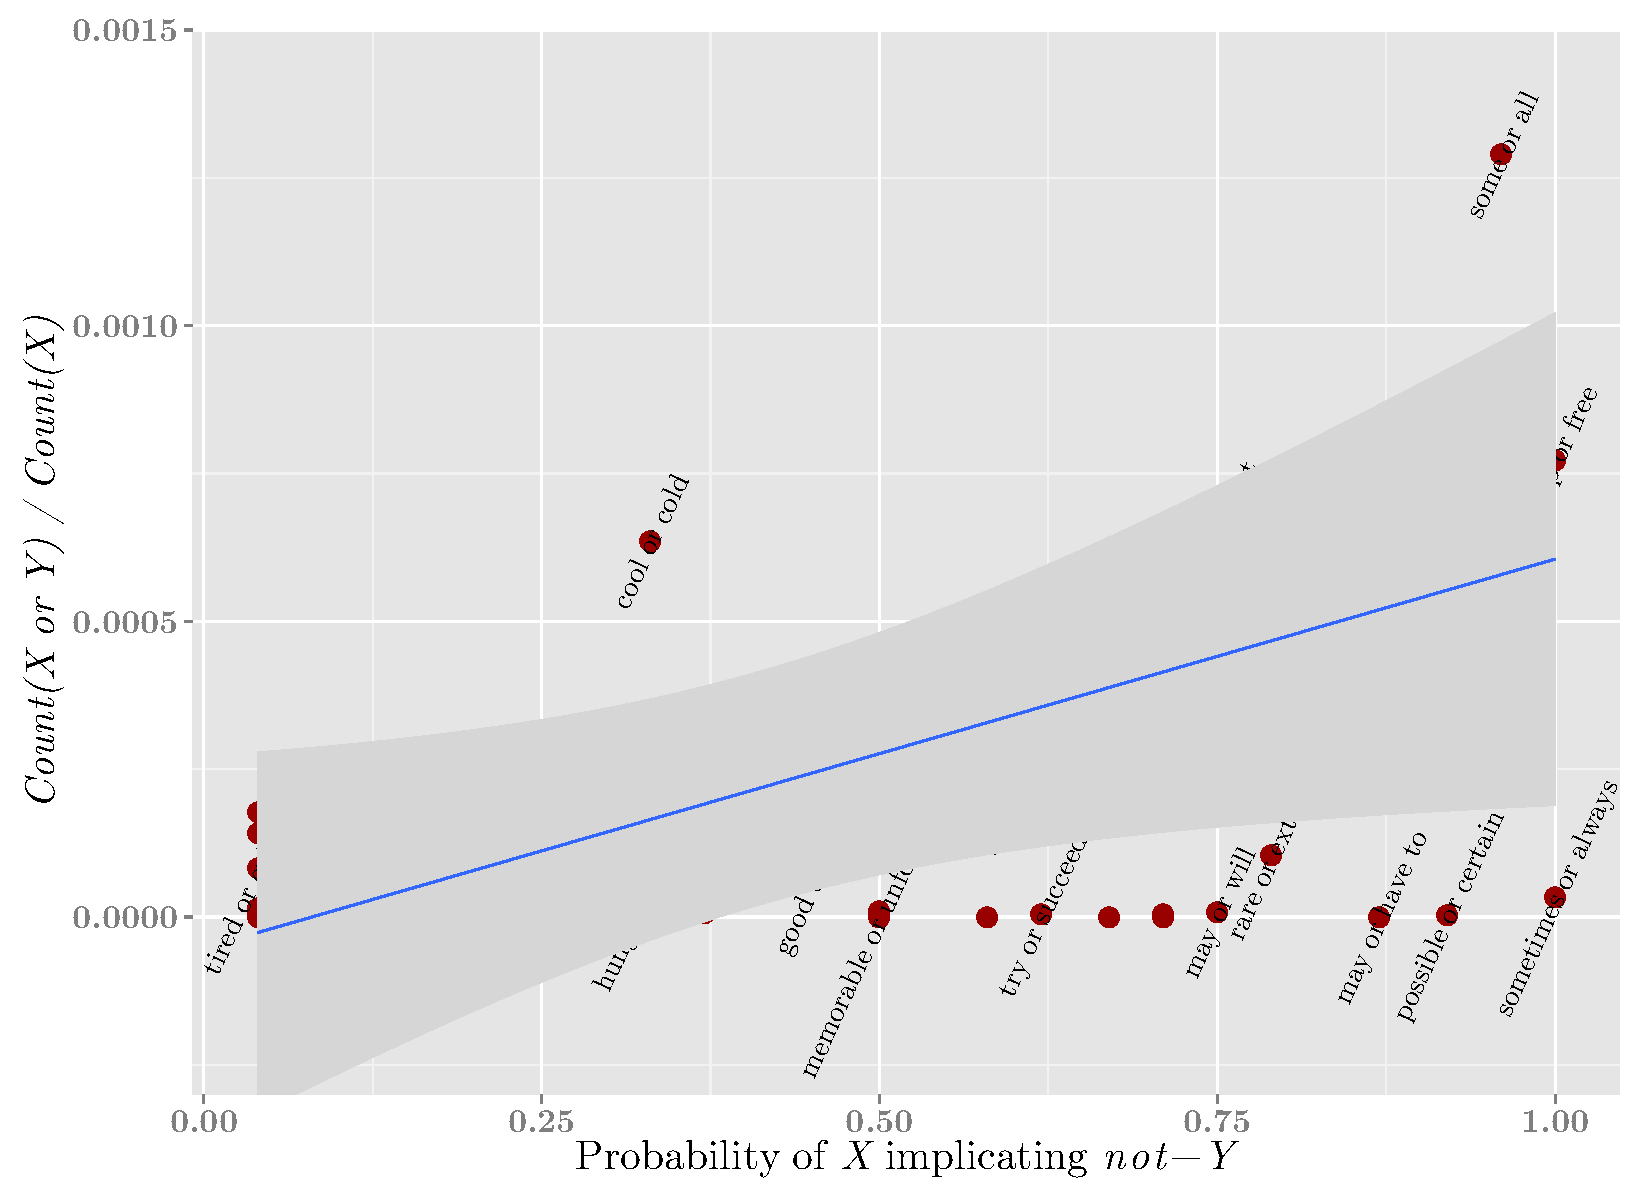
\includegraphics[width=0.7\textwidth]{fig/disjunction-and-implicature}
  \caption{The relative frequency of \word{X or Y} is predicted by the
    probability of $X$ implicating \word{not Y}.  All the data points
    are given (red dots) and included in the analysis. For the sake of
    readability, only a subset of the associated disjunctions are
    printed.}
  \label{fig:chemla}
\end{figure}

Blocking a potential scalar implicatures is just one of the
motivations a speaker might have for uttering a disjunction that
superficially violates HG. The I-implicatures studied by
\citet{Levinson00} can also be motivating factors: the speaker is
compelled to say as a little as possible, and the listener is advised
to seek out specific interpretations. As a corollary of this, general
terms are often prone to being restricted to salient or prototypical
subkinds. For instance, at a busy marina in water-skiing country,
\word{boat} might come to identify just motorboats. In that context, a
speaker wishing to state a rule or regulation about all watercraft
might use \word{boat or canoe} or \word{boat or kayak} to ensure that
these non-motorized cases are included, lest people assume (or feel
licensed to act as if they can assume) that these rarer kinds of boat
are exempt.

%\marginpar{I cut the country/capital data, but it could be added. Even though it is sparse, it contains interesting patterns relating to the frequency of the two terms and the ratios of their frequencies. (E.g., low ratios correlate with disjunction usage).}

% Eager for a more rigorous assessment of the prevalence of
% HG-violating disjunctions, we conducted a simple experiment. First,
% we obtained a list of countries and their capitals and, to keep the
% search procedure simple, extracted the subset in which the country
% and capital both have single word names. Second, we searched for
% `\emph{country or capital}' and `\emph{capital or country}' in the
% Google Books N-grams data, restricting attention to books after 1960
% to try to avoid some of the encoding difficulties that plague
% earlier texts in that corpus. Of the 128
% $\set{\word{`country'}, \word{`capital'}}$ cases in which both
% \word{`country'} and \word{`capital'} are attested in the data, 11
% are attested in the form \word{`country' or `capital'} and 11 are
% attested in the form \word{`capital' or `country'}. The two sets are
% nearly coextensive.

In these implicature-blocking scenarios, the speaker is concerned that
the general term \word{X} will be construed as
$\sem{\word{X\/}}-\sem{\word{Y\/}}$ for some $\sem{\word{Y\/}}$
overlapping with $\sem{\word{X\/}}$, and the disjunction hedges
against that possibility. This is a \technicalTerm{defensive} position; the speaker's
own lexicon might allow her to use just the general term to convey her
intentions, but she is concerned that the listener will arrive at a
different conclusion. The costs of disjunction are therefore worth
paying even if the disjunction adds no new information given the
speaker's lexicon.  However, the speaker can play a more active role
as well, using disjunctions to instruct the listener about the right
lexicon. Our \secref{sec:introduction} example containing
``angioplasty or surgery'' seems to be an instance of this: the
disjunction conveys secondary information that \word{angioplasty} and
\word{surgery} will be treated as separate options in the discourse
\citep{Simons:2001}. If HG were adopted as an explicit theoretical
constraint, then the possibility of doing this would more or less
follow --- we just require the additional premise that the listener is
charitable and so will try to find an acceptable construal of the
utterance. The model we develop in \secref{sec:model} also supports
this kind of reasoning, but it requires no independent statement of
HG.
 
%=====================================================================

\subsection{Definition and identification}\label{sec:data:definitional}

Disjunctions like \word{wine lover or oenophile} seem to fly in the
face of the Hurfordian pressure reviewed just above. Rather than
avoiding overlap, they seem to embrace it, conveying something
approximating identity.

Definitional disjunctions are even more contextually restricted than
HG-violating disjunctions, so generalizing about their usage
conditions is difficult.  The examples in \eg{ted} were obtained by
annotating the disjunctive clauses in a sample of 98 TED talks. These
talks seem ideal for finding definitional uses, because the speakers
are experts with broadly pedagogical aims. In addition, videos of the
talks are available online, which made it possible for us to use
intonation and other cues to try to verify that the speakers had
definitional intentions. These seven examples were drawn from a set of
344 disjunctive clauses, for a rate of only about 2\%, despite the
context being conducive to such uses. The examples are given with the
punctuation from the transcripts that TED provides.
%
\begin{exe}
  \ex\label{ted}
  \begin{xlist}
    \ex \ldots more disorder, or ``entropy,'' over their lifetimes 
    
    (Alex Wisssner Gross, `A new equation for intelligence', 5:51)

    \ex \ldots by the gametes, or the sperm and the eggs.

    (Carin Bondar, `The birds and the bees are just the beginning', 3:02)

    \ex This is Toxoplasma gondii, or Toxo, for short, \ldots

    (Ed Yong, `Zombie roaches and other parasite tales', 9:33)

    \ex the Carnegie Airborne Observatory, or CAO

    (Greg Asner, `Ecology from the air', 2:22)

    \ex We call this project VocaliD, or vocal I.D., \ldots

    (Rupal Patel, `Synthetic voices, as unique fingerprints', 3:52)

    \ex they can self-renew or make more of themselves \ldots

    (Siddharthan Chandran, `Can the damaged brain repair itself?', 8:05)

    \ex the endogenous stem cells, or precursor cells,

    (Siddharthan Chandran, `Can the damaged brain repair itself?', 14:48)
  \end{xlist}
\end{exe}

As these examples suggest, speakers often (but not always) signal
definitional intentions with ad hoc prosody, italics, quotation marks,
and other devices, which points to the marked nature of the
usage. However, it would be a mistake to dismiss definitional uses as
an idiosyncrasy of English. These uses are widely attested in
typologically diverse languages (we have examples from Chinese,
German, Hebrew, Ilokano, Japanese, Russian, and Tagalog). Even
languages that seem to have a dedicated `definitional' or
`metalinguistic \word{or}' (e.g., Finnish, Italian) seem also to allow
the regular \word{or} to play this role.

For our purposes, the most important property of these uses is that
they convey a meaning that is secondary to the main content of the
utterance --- an extreme instance of a meaning that is not at-issue
\citep{Tonhauser-etal:2011,Dillon-etal:2014}. This contrasts with
overt definitions like \word{`oenophile' means `wine-lover'} or
\word{oenophile: wine-lover} (in a dictionary context).  We think it
is no accident that another strategy for conveying definitional
information in this non-asserted, taken-for-granted manner is via
apposition, as in \word{oenophile (`wine-lover')}, since appositives
too are often recruited to convey secondary, supporting information
\citep{Potts05BOOK,Potts08HSK,Syrett-etal:2014}. In this respect, the
relevant inference resembles the exclusivization pressure identified
by HG: both seem to emerge as side-effects rather than normal
outputs. In our model (\secref{sec:model}), both are in turn
characterized as ``meta-linguistic'' --- inferences about the lexicon
rather than about the state of the world.

In addition, as with disjunct exclusivization, the relevant lexical
inference might be temporary. For instance, phrases like
\word{Internet or computer network} seem to use the second phrase as a
rough-and-ready way of helping the listener bootstrap towards an
understanding of what the Internet is. Even our wine-lover example
involves only approximate synonymy; according to our
intuitions,\word{wine lover or oenophile} seems apt in a context in
which the speaker wishes to use \word{oenophile} to elevate the
concept to something more specific (or pretentious) than \word{wine
  lover} picks out. Similarly, the book title \emph{A Geological
  History of Manhattan or New York Island} identifies Manhattan with
New York Island while at the same time acknowledging the different
histories and connotations of the two disjuncts.

The speaker's motivations for using definitional disjunction are
varied. Such readings seem to arise most easily when the speaker is
mutually and publicly known to have \technicalTerm{expertise} in the
domain covered by the terms and the listener is mutually and publicly
known to be inexpert in that area. In such cases, the speaker can use
the disjunction to convey information about her preferred lexicon,
fairly certain that the listener will be receptive. However, while
speaker expertise seems to be a genuine prerequisite, the listener's
knowledge seems to impose little on felicitous uses. We find natural
uses of this strategy when there is no direct information about the
listener, but rather just a general assumption that one of the terms
is relatively unknown. For instance, a newspaper article might contain
\word{wine lover or oenophile} without presuming that all its readers
are ignorant of the terms; rather, such a use would seem to presuppose
only that \word{oenophile} is relatively unknown, or obscure enough
that it's useful to reinvoke its definition. At the the other end of
the spectrum, the listener might actually be presumed to know the
term, but the speaker sees social value in conveying that she shares
this view. This could be because the speaker would like to display
expertise, as when an ambitious student seeks to convey competence to
a professor. The uses also arise when the speaker and listener might
both be experts in the domain and see value (jointly or just in the
current speaker's eyes) in using a word in a specialized sense in
order to name a concept efficiently (e.g., the hypothetical academic
paper title \word{What motivates the snobbish wine lover or
  `oenophile' and how does he differ from the casual drinker?}).

For these reasons, we propose the following, more general set of
desiderata that we believe must hold in order for definitional
interpretations to be licensed.  First, the discourse participants
must have a mutual interest in communicating not only about the world
but also about their language and arriving at a refined -- even if
context-specific and fleeting -- joint understanding of it. Second,
the discourse participants should share as a background assumption
that the speaker and listener are willing to coordinate on the lexicon
that the speaker seems to be using.  That is, there must be tacit
agreement between speaker and listener that utterance interpretation
can proceed on the assumption of speaker expertise in the language of
the domain of the conversation.  Third and finally, the cost of using a
disjunction must be fairly small, all things considered, else it is
hard to see how the speaker could justify using a disjunction \word{X
  or Y} to convey simply $\sem{\word{X\/}}$.  That is, whatever the
costs of using the verbose form, they must be worth paying in virtue
of the benefits of identifying (for the purposes of the current talk
exchange) the meanings of the two disjuncts.

%%%%%%%%%%%%%%%%%%%%%%%%%%%%%%%%%%%%%%%%%%%%%%%%%%%%%%%%%%%%%%%%%%%%%%

\section{Modeling communication with under conditions of speaker expertise}\label{sec:model}

We now describe our model of pragmatic reasoning. Our presentation is
somewhat compact. Readers wishing to more fully explore the model are
referred to the website for this paper, which provides implementations
of this model (as well as those of \citealt{Frank:Goodman:2012},
\citealt{bergen-levy-goodman:2014}, and
\citealt{Smith:Goodman:Frank:2013}) and includes code for calculating
all of the examples we review here.

In our model, production and interpretation are based in a recursive
process in which speaker and listener agents reason about each other
reasoning about each other.  At the lowest levels of our model, these
agents communicate using a single lexicon. However, we do not actually
assume that a single lexicon is mutually and publicly recognized as
the set of core conventions of the language. Rather, our model
aggregates over many possible lexica, thereby allowing the agents to
negotiate the structure of the language itself even as they
communicate. \Figref{fig:modstruc} summarizes this picture
schematically; this section is devoted to explicating these agents and
their relationships.

\begin{figure}[tp]
  \centering
  \newcommand{\labelednode}[2]{\put(#1){\makebox(0,0){#2}}}
  \newcommand{\picarrow}[3][0.9]{\put(#2){\vector(#3){#1}}}
  \newcommand{\picdownarrow}[1]{\picarrow{#1,0.8}{-3,-2}}
  \newcommand{\picuparrow}[1]{\picarrow{#1,0.2}{-3,2}}
  \setlength{\unitlength}{1cm}
  \begin{picture}(8,1.5)
    \labelednode{1,1.5}{\textbf{Fixed $\Lex$}}
    \labelednode{5.5,1.5}{\textbf{Reasoning about possible $\Lex$}}
    \labelednode{0,1}{$\listenerZero$}
    \picuparrow{1}
    \labelednode{1,0}{$\speakerOne$}
    \picdownarrow{2}
    \labelednode{2,1}{$\listenerOne$}
    \picarrow[0.7]{2.8,1}{-1,0}
    \labelednode{3,1}{$\ListenerK[1]$}
    \picuparrow{4}
    \labelednode{4,0}{$\SpeakerK[2]$}
    \picdownarrow{5}
    \labelednode{5,1}{$\ListenerK[2]$}
    \picuparrow{6}
    \labelednode{6,0}{$\SpeakerK[3]$}
    \picdownarrow{7}
    \labelednode{7,1}{$\ListenerK[3]$} 
    \picuparrow{8}
    \labelednode{8,0}{$\ldots$}
  \end{picture}
  \caption{Summary of model structure.}
  \label{fig:modstruc}
\end{figure}

The core structures of our model are given in \eg{model}.
Intuitively, we imagine that a speaker and listener are playing a game
in which the speaker privately observes a state $\state \in \States$
and produces a message $\msg \in \Messages$ on that basis, given the
context defined by the signaling system. The listener then uses $\msg$
to guess a state $\state' \in \States$. The communication is
successful just in case $\state = \state'$. The agents that we define
are rational in the sense that, by reasoning recursively about each
other's behaviors, they can increase their chances of success at this
signaling game.
%
\begin{exe}
\ex\label{model}
  \begin{xlist}
  \ex\label{states}%
    $\States$ is a set of states (worlds, referents, propositions, etc.).
  \ex\label{messages}%
    $\Messages$ is a set of messages containing designated `null' message $\nullmsg$.
  \ex\label{lex}%
    $\LexStar: \Messages \mapsto \wp(\States)$ is a semantic interpretation function. 
    $\Lex'(\nullmsg) = \States$.
  \ex\label{prior}%
    $\Prior : \States \mapsto [0,1]$ is a prior probability
    distribution over states.    
  \ex\label{costs}%
    $\Costs : \Messages \mapsto \Reals$ is a cost function on messages.
    %$\Costs(\nullmsg) > \Costs(\msg), {\forall \msg \in \Messages{-}\set{\nullmsg}}$.
  \end{xlist}
\end{exe}

Clause~\subeg{model}{messages} designates a null message $\nullmsg$
and clause~\subeg{model}{lex} includes a stipulation that $\nullmsg$
is true in all states in all lexica. It can be thought of as a
catch-all for the numerous messages in the language that are not
discriminating in the context defined by the signaling system.  No
matter how big and complex the examples, such a message is always
justified. Introducing $\nullmsg$ also helps ensure that various
calculations in the model are well-defined. (For alternative methods
of ensuring definedness, see \citealt{Jaeger:2011} and
\citealt{bergen-levy-goodman:2014}.)

%=====================================================================

\subsection{Simple state/message signaling}\label{sec:rsa}

As \figref{fig:modstruc} shows, our model defines an intuitive hierarchy
of agents. The most basic are $\listenerZero$, $\speakerOne$, and
$\listenerOne$. These agents reason in terms of a fixed lexicon
$\Lex$, which, for our purposes, can be thought of as a standard
semantic interpretation function, as in \subeg{model}{lex}. These
agents suffice to define a version of the Rational Speech Acts model
of \citet{Frank:Goodman:2012} and \citet{Goodman:Stuhlmuller:2013}.

The starting point is $\listenerZero$. This agent simply turns $\Lex$
into a probabilistic formulation that can be used for decision-making
in the presence of communicative indeterminacy. The first term defines
an even distribution over all of the true states $\state$ for the
given message $\msg$, and the second term incorporates the contextual
prior distribution over states $\Prior$. (Here, $\Indicator$ is an
indicator function: $\Indicator(\varphi) = 1$ if $\varphi = \True$,
else $0$.)
%
\begin{exe}
\ex\label{l0} $\listenerZero(\state \given \msg, \Lex) \propto \frac{\Indicator(\state \in \Lex(\msg))}{|\Lex(\msg)|} \Prior(\state)$
\end{exe}

This agent is pragmatic only insofar as it incorporates the contextual
prior into (a distribution derived from) the truth conditions. Richer
pragmatic inferences start to emerge as soon as we envision a speaker
that can reason in terms of this listener and plan its utterances
accordingly. The minimal such speaker is $\speakerOne$, which is
defined in terms of $\listenerZero$:
%
\begin{exe}
\ex\label{s1} $\speakerOne(\msg \given \state, \Lex) \propto \exponential \left( \alpha\log \left( \listenerZero(\state \given \msg, \Lex) \right) -  \Costs(\msg) \right)$
\end{exe}
%
This definition is a bit cumbersome because of the need to ensure that
all values are positive even with real-valued costs. At its heart,
though, this agent is parallel to $\listenerZero$ in that it combines
a conditional distribution and a piece of contextual information ---
now costs on messages. The result is a distribution that one can
imagine serving as the basis for decision making: given that the agent
would like to convey that a certain state holds, which message will do
that most effectively for the $\listenerZero$ listener? The
real-valued parameter $\alpha$ controls the degree to which the
speaker tries to capitalize on the distinctions $\listenerZero$
encodes.

The first pragmatic listener is $\listenerOne$. It is parallel to
$\listenerZero$ except that it reasons, not in terms of the original
lexicon, but rather in terms of $\speakerOne$ reasoning about
$\listenerZero$ reasoning about the lexicon. This agent is essentially
a derived, pragmatically-enriched probabilistic interpretation
function:
%
\begin{exe}
\ex\label{l1} $\listenerOne(\state \given \msg, \Lex) \propto \speakerOne(\msg \given \state, \Lex) \Prior(\state)$
\end{exe}

\Figref{fig:rsa-disj} shows how this model derives basic scalar
implicatures. We've used disjunction to illustrate, but the reasoning
holds wherever general terms compete with more specific (entailing or
merely overlapping) ones. In terms of the communication game, suppose
the speaker produced the message $\porq$. For the literal listener
$\listenerZero$, all three worlds have equal probability given this
message, making it unlikely that the two agents will succeed in
communication. However, the first pragmatic listener $\listenerOne$,
reasoning in terms of $\speakerOne$, has a greater chance of success.
It has already learned to separate the related terms: $\porq$ conveys
that $\pandq$ is false, and the atomic propositions convey biases not
present in their disjunction. One can also see that the speaker seeks
to avoid ambiguities. For instance, where an atomic proposition is
true, the speaker opts for it, thereby creating less uncertainty in
the listener than a disjunction would.

This basic model has been shown to achieve good quantitative fits to
experimental results
\citep{Degen:Franke:2012,Stiller:Goodman:Frank:2011} and to contribute
to artificial agents that communicate effectively with each other to
solve a collaborative task \citep{Vogel-etal:2013}. One can also
generalize $\listenerOne$ and $\speakerOne$ to allow them to
recursively respond to each other, which strengthens the scalar
inferences seen in \figref{fig:rsa-disj}. In our model, there is no
further recursion of these lexicon-specific agents, but we do allow
further recursion of the agents we define next.

\begin{figure}[tp]
  \centering
  \setlength{\arraycolsep}{3pt} 
  $\begin{array}[b]{c c r@{\hspace{25pt}}l}
     \listenerMatrix%
     {\LexStar}%
     {\True & \True  & \False}%
     {\True & \False & \True}%     
     {\True & \False & \False}%  
     {\True & \True  & \True}% 
     {\True & \True  & \True}%  
     &
     \longleftarrow
     &
     \listenerMatrix%
     {\listenerZero}%
     { .5 &  .5 &   0}%
     { .5 &   0 &  .5}%
     {1   &   0 &   0}%     
     {.33 & .33 & .33}%
     {.33 & .33 & .33}%
     &
     \listenerMatrix%
     {\listenerOne}%
     { .3 & \graycell{.7} &   0}%
     { .3 &   0 & \graycell{.7}}%
     {\graycell{1} &   0 &   0}%     
     { .17 & \graycell{.41} & \graycell{.41}}%
     { .17 & \graycell{.41} & \graycell{.41}}%
   \\
   && \nwarrow & \swarrow
   \\
   &&
   \multicolumn{2}{c}{
      \speakerMatrix%
      {\speakerOne}%
      {.33 & .33 & .25 & .08 & 0}%
      {.8 & 0   &   0 & .2 & 0}%
      {  0 & .8 &   0 & .2 & 0}%
   }
   \end{array}$   
   \caption{Simple state/message signaling with disjunction. 
     $\Prior(w_{i}) = 1/3$ for all states $w_{i} \in \States$,
     $\Costs(\word{or}) = \Costs(\word{and}) = 1$, and 
     $\alpha = 1$. 
     Listener $\listenerOne$'s best inferences are in gray. 
     The recursive process separates disjunction and conjunction, and 
     it also separates disjunction from each of its disjuncts.}
  \label{fig:rsa-disj}
\end{figure}

%=====================================================================

\subsection{Reasoning under lexical uncertainty}\label{sec:full}

In the model defined by $\listenerZero$, $\speakerOne$, and
$\listenerOne$, the agents condition on (take as given) a fixed,
shared lexicon. However, the data in \secref{sec:data} show that the
lexicon is not known precisely, but rather negotiated during
interactions. We now bring that insight into our model using the
lexical uncertainty technique first introduced by
\citet{Bergen:Goodman:Levy:2012,bergen-levy-goodman:2014}. The first
step is to define a space of lexica $\LexSet$ and a probability
distribution over them $\LexPrior$:
%
\begin{exe}
\ex\label{model-extend}
  \begin{xlist} 
  \ex\label{lexset}%
      $\LexSet = 
      \set{\Lex' : 
        \Lex'(\nullmsg) = \States \mathbin{\&}
        \forall \msg \in \Messages{\negthinspace-\negthinspace}\set{\nullmsg}, 
        \Lex'(\msg) \neq \emptyset \mathbin{\&}
        \Lex'(\msg) \subseteq \LexStar(\msg)}$
  \ex\label{LexPrior}% 
    $\LexPrior : \LexSet \mapsto [0,1]$ is a prior
    probability distribution over lexica.  
  \end{xlist}
\end{exe}
%
Clause~\subeg{model-extend}{lexset} defines a complete set of
refinements of a basic lexicon: every lexical item can denote a subset
of the space it denotes in the base lexicon $\LexStar$, and all
combinations of these refinements are available. The only requirements
are that messages always have non-empty denotations and that the null
message $\nullmsg$ always denotes the full set of states. The
resulting definition gives us an intuitive, computationally manageable
space to work with. We should emphasize, though, that these
assumptions are not essential to our model. In the extreme case, we
could admit every lexicon derivable from the messages $\Messages$ and
states $\States$, and then use the lexicon prior $\LexPrior$ to
provide some structure to the space --- say, by assigning low but
non-zero probability to lexica that are not strict refinements, and
zero probability to lexica in which $\nullmsg$ is not universal or
some messages have empty denotations. This is a strictly more general
perspective than the one given by \eg{model-extend}. We do not explore
these options further in this paper, but see
\citealt{Kao:Bergen:Goodman:2014,Kao-etal:2014} and for discussion of
non-refinement pragmatic enrichment involving non-literal language.

Our first `lexical uncertainty' agent is $\ListenerK[1]$, which is
based on the model of \citet{Smith:Goodman:Frank:2013}. Given a
message, this agent makes joint lexicon--state inferences from
the space $\States \times \LexSet$:
%
\begin{exe}
  \ex\label{L1}%
    \setlength{\arraycolsep}{2pt}%  
    $\begin{array}[t]{@{} r c l}
      \ListenerK(\state, \Lex \given \msg) 
      &=&
      \ListenerK(\state \given \msg, \Lex) \ListenerK(\Lex \given \msg) 
      \\[1ex]
      \ListenerK(\Lex \given \msg) 
      &\propto& 
      \Prior(\Lex) \sum_{\state\in\States} \SpeakerK(\msg \given \state, \Lex)\Prior(\state)
    \end{array}$
\end{exe}
%
This agent is defined for levels $k \geqslant 1$ as long as we assume
that $\SpeakerK[1] = \speakerOne$ (higher levels use the speaker in
\eg{Sk}) and
$\ListenerK[1](\state \given \msg, \Lex) = \listenerOne(\state \given
\msg, \Lex)$.
The first term uses a fixed-lexicon inference and the second encodes
the extent to which the current message biases in favor of the lexicon $\Lex$.

Our `expertise' speaker responds to this lexical uncertainty listener.
We assume that this speaker does have a specific lexicon in mind (this
is the sense in which it is expert).  More precisely, this speaker is
taken to observe state--lexicon pairs and produce messages on that
basis. It is defined for all $k > 1$:

\begin{exe}  
  \ex\label{Sk}%
   $\SpeakerK(\msg \given \state, \Lex) \propto \exponential \left( \alpha\log\left(\ListenerK[k-1](\state \given \msg, \Lex)\right)  -  \beta\log\left(\ListenerK[k-1](\Lex\given\msg)\right) - \Costs(\msg) \right)$
\end{exe}
%
In broad terms, this agent is similar to $\speakerOne$ except that it
includes a new term $\ListenerK[k-1](\Lex\given\msg)$ encoding the
information each message conveys about the lexicon. The relative
importance of this information is controlled by a new real-valued
learning-rate parameter $\beta$. The relative weights of $\alpha$ and
$\beta$ control the relative importance of conveying information about
the world and information about the lexicon, and much of our
investigation of disjunction focuses on this relationship.

Let's return to the schematic diagram in
\figref{fig:modstruc}. Intuitively, if one begins at, say,
$\ListenerK[2]$, then the reasoning flows down through the uncertainty
agents $\SpeakerK[2]$ and $\ListenerK[1]$, at which point it splits
apart into lower-level agents that reason about specific lexica.
Alternatively, one can imagine the lexicon-specific inferences flowing
up to be pooled together by $\ListenerK[1]$, which then makes joint
inferences about the state and the lexicon.

\Figref{fig:simple-example} seeks to show how the model works with a
simple case involving a scalar inference. In the figure, the bottom
row specifies the lexica defined by \subeg{model-extend}{lexset} with
$\LexStar$ as the starting point; the more specific term has no
further refinements, but the general term has two further refinements,
resulting in three lexica. The lexicon-specific agents
$\listenerZero$, $\speakerOne$, and $\listenerOne$ reason about these
lexica. At the $\ListenerK[1]$ level, we have given just the joint
table for the message \word{cheap}, but there are similar tables for
the messages \word{free} and $\nullmsg$. Similarly, we've given only
one conditional probability table for $\SpeakerK[2]$; there are
similar tables for $\LexStar$ and $\Lex_{1}$. Finally, we depict the
\word{cheap} table for $\ListenerK[2]$. For this example, we set
$\alpha = 1$ and $\beta = 2$. The relatively large $\beta$ parameter
means that the speaker values communicating about the lexicon, and we
can see the effects of this in $\ListenerK[2]$, which displays a
dispreference for $\Lex_{1}$, equivalently, a preference for the
lexica that distinguish \word{cheap} from \word{free}. More generally,
even in this basic example, $\ListenerK[2](\Lex\given\msg)$
discriminates among lexica, meaning that this agent can use
$\SpeakerK[2]$'s message to gain insights into its lexical
preferences. If $\beta$ is lowered, then this becomes less pronounced,
and $\beta = 0$ means that $\ListenerK[2](\Lex\given\msg)$ becomes
flat (treats all lexica as identical).

\begin{figure}[htp]
  \centering
  \renewcommand{\arraystretch}{0.9}

  \newcommand{\singlearrowdivider}{& \multicolumn{3}{c}{\downarrow}}
  \newcommand{\straightarrowdivider}{& \downarrow & \downarrow & \downarrow}
  \newcommand{\angledarrowdivider}{& \multicolumn{3}{c}{\swarrow \hspace{75pt} \downarrow\hspace{75pt} \searrow}}

  \setlength{\arraycolsep}{12pt}
  $\begin{array}[c]{r@{\mspace{10mu}}c c c}
  \ListenerK[2] & \multicolumn{3}{c}{\examplejoint{\text{heard }\word{cheap}}{.12 & \graycell{.29}}{.04 & .22}{.04 & \graycell{.29}}}
  \\
  \singlearrowdivider
  \\
  \SpeakerK[2] & \multicolumn{3}{c}{\exampleSpeaker{\text{prefers } \Lex_{2}}{.15 & .85 & 0}{1 & 0 & 0}}
  \\
  \singlearrowdivider
  \\
  \ListenerK[1] & \multicolumn{3}{c}{\examplejoint{\text{heard }\word{cheap}}{.12 & .35}{.18 & 0}{0 & .35}}
  \\
  \angledarrowdivider
  \\
  \listenerOne & \examplelistener{.25 & .75}{1 & 0}{.25 & .75} & \examplelistener{1 & 0}{1 & 0}{0 & 1} & \examplelistener{0 & 1}{1 & 0}{.5 & .5}
  \\
  \straightarrowdivider
  \\
  \speakerOne & \examplespeaker{.33 & .67 & 0}{.99 & 0 & .01} & \examplespeaker{.5 & .5 & 0}{0 & 0 & 1} & \examplespeaker{0 & 1 & 0}{1 & 0 & 0}
  \\
  \straightarrowdivider
  \\
  \listenerZero & \examplelistener{.5 & .5}{1 & 0}{.5 & .5} & \examplelistener{1 & 0}{1 & 0}{.5 & .5} & \examplelistener{0 & 1}{1 & 0}{.5 & .5}
  \\
  \straightarrowdivider
  \\
  \Lex & \examplelex[\LexStar]{\True & \True}  & \examplelex[\Lex_{1}]{\True & \False} & \examplelex[\Lex_{2}]{\False & \True}
  \end{array}$                                                                                          
  \caption{Illustration of the full model in action. 
    The priors over worlds and lexica are all flat, 
    message costs are all $0$,
    $\alpha=1$, and 
    $\beta=2$. 
    The high $\beta$ means that $\ListenerK[2]$ shows a notable dispreference for the undiscriminating lexicon $\Lex_{1}$.}
  \label{fig:simple-example}
\end{figure}

%=====================================================================

\subsection{A return to simple signaling}\label{sec:return}

The full model can be unwieldy because of the lexicon inferences.  One
often wants to return to the intuitive picture of simple state/message
signaling, as in examples like \figref{fig:rsa-disj}. To achieve this,
one can sum over lexica, as in \eg{lisnorm} and \eg{spknorm}. Both
provide useful summaries of the model's predictions.
%
\begin{exe}
\ex\label{lisnorm} $\ListenerK(\state \given \msg)  = \sum_{\Lex \in \LexSet} \ListenerK(\state, \Lex \given \msg)$
\ex\label{spknorm} $\SpeakerK(\msg \given \state) \propto \sum_{\Lex \in \LexSet} \SpeakerK(\msg \given \state, \Lex) \LexPrior(\Lex)$
\end{exe}
%
\Figref{fig:marginalized} uses these equations to summarize the
inferences for $\ListenerK[2]$ and $\SpeakerK[2]$ from
\figref{fig:simple-example}. We no longer get insights into the
agents' lexical preferences and inferences, but we do see that they
are computing scalar inferences in the manner we saw for the simpler
model in \figref{fig:rsa-disj}.

\begin{figure}[tp]
  \centering
  \begin{subfigure}[b]{0.4\textwidth}
    \centering
    $\examplelistener{.2 & \graycell{.8}}{\graycell{1} & 0}{0 & \graycell{1}}$
    \caption{$\ListenerK[2]$}
  \end{subfigure}
  \qquad
  \begin{subfigure}[b]{0.4\textwidth}
    \centering
    $\examplespeaker{.23 & \graycell{.77} & 0}{\graycell{.92} & 0 & .08}$
    \caption{$\SpeakerK[2]$}
  \end{subfigure}
  \caption{Return to simple signaling for the simple scalars example
    in \figref{fig:simple-example}.}
  \label{fig:marginalized}
\end{figure}

%%%%%%%%%%%%%%%%%%%%%%%%%%%%%%%%%%%%%%%%%%%%%%%%%%%%%%%%%%%%%%%%%%%%%%

\section{Compositional lexical uncertainty}\label{sec:composition}

There are two shortcomings of the model as presented so far that are
important to correct before studying Hurfordian and definitional usage
patterns. Both of these shortcomings are evident in the treatment of
disjunction in \figref{fig:rsa-disj}.

First, if we took the lexicon given there as the base lexicon and
applied lexical uncertainty to it using \subeg{model-extend}{lexset},
the results would be highly unintuitive because many lexica would fail
to respect the desired semantic relationships that hold among the
messages. For example, there would be lexica in which $\porq$ strictly
entailed $p$. The culprit here is that lexical uncertainty, applied
naively, does not respect compositional semantics.  To address this,
we follow \citet{bergen-levy-goodman:2014} and
\citet{levy-bergen-goodman:2014SALT} in applying uncertainty only to
the true lexical items, and then close each lexicon under the
compositional operations of disjunction and conjunction. Thus, in
\figref{fig:rsa-disj}, only $p$ and $q$ can be refined.  This results
in nine distinct lexica.  Each of these is then expanded to include
$\pandq$ and $\porq$, with their meanings determined by whatever
meanings the atomic expressions have.  

\begin{figure}[tp]
  \centering
  \newcommand{\labelednode}[2]{\put(#1){\makebox(0,0){#2}}}
  \newcommand{\picline}[3]{\put(#1){\line(#2){#3}}}
  \setlength{\unitlength}{1cm}
  \begin{picture}(5.5,2)   
    \labelednode{0.5,2}{$w_{1}$}
    \labelednode{2.75,2}{$w_{2}$}
    \labelednode{5,2}{$w_{3}$}
    
    \picline{0.5,1.2}{0,1}{0.6}
    \picline{0.75,1.2}{3,1}{1.8}
    \labelednode{0.5,1}{$w_{1} \vee w_{2}$}
        
    \picline{2.5,1.2}{-3,1}{1.8}
    \picline{3.0,1.2}{3,1}{1.8}
    \labelednode{2.75,1}{$w_{1} \vee w_{3}$}

    \picline{5,1.2}{0,1}{0.6}
    \picline{4.75,1.2}{-3,1}{1.8}
    \labelednode{5,1}{$w_{2} \vee w_{3}$}
    
    \picline{2.5,0.2}{-3,1}{1.8}
    \picline{2.75,0.2}{0,1}{0.6}
    \picline{3.0,0.2}{3,1}{1.8}
    \labelednode{2.75,0}{$w_{1} \vee w_{2} \vee w_{3}$}
  \end{picture}
  \caption{State space with disjunctive closure.}
  \label{fig:closure}
\end{figure}

Second, the world space in \figref{fig:rsa-disj} does not create any
room for the speaker to be uncertain. The pretense is that the speaker
always observes the state perfectly (up to the level of granularity
being measured) and then seeks to communicate that observation. This
gives somewhat unintuitive results for disjunction. Disjunction is
naturally used to convey speaker uncertainty, but we currently allow
no room for such uncertainty.  To address this, we close the state
space under joins.  For the set of atomic states
$\set{w_{1}, w_{2}, w_{3}}$, this results in the semilattice in
\figref{fig:closure}. Interpretation via $\Lex$ then proceeds as one
would expect: disjunction corresponds to union and conjunction to
intersection. For example, if $\Lex(p) = \set{w_{1}, w_{2}}$ and
$\Lex(q) = \set{w_{1}, w_{3}}$, then
$\Lex(\porq) = \set{w_{1}, w_{2}, w_{3}}$.  After join closure, this
denotes the entire state space represented in
\figref{fig:closure}. Conversely, $\pandq$ denotes $\set{w_{1}}$,
which does not change under closure. (We could expand the space of
meanings to include meets, or even to the full Smyth powerlattice with
states like $w_{1}{\vee} (w_{2}{\wedge} w_{3})$, as in
\citealt{levy-pollard:2001}, but we stick with the join space to keep
the presentation as simple as possible.)

Formally, the model we have developed here is an instance of the
compositional lexical-uncertainty model of
\citet{bergen-levy-goodman:2014} and
\citet{levy-bergen-goodman:2014SALT}, with two elaborations: we have
placed value on transmission of the lexicon from speaker to listener
(Equation~\ref{Sk}) and specified the structure of world state space
for the classes of utterances presently under consideration.
\Figref{fig:compdisj} summarizes how our model behaves in this
setting. We begin from a base lexicon $\LexStar$ in which $\LexStar(p)
= \set{w_{1}, w_{2}}$ and $\LexStar(q) = \set{w_{1}, w_{3}}$. We apply
lexical uncertainty to obtain nine distinct lexica, close their state
space under joins, and close their messages under disjunction and
conjunction. We run the full model up to level $\ListenerK[2]$, and
then marginalize $\ListenerK[2]$ and $\SpeakerK[2]$ as in \eg{lisnorm}
and \eg{spknorm}, respectively. The results are closely aligned with
the comparable tables in \figref{fig:rsa-disj}, in that we obtain all
of the interpretive scalar implicatures and predict largely the same
speaker behavior. The one major improvement is that we now directly
capture the intuition that disjunction can signal speaker uncertainty:
the speaker's best choice for state $w_{2}{\vee}w_{3}$ is $\porq$.

\begin{figure}[tp]
  \centering
  \begin{subfigure}{1\textwidth}
    \centering
    $\closurelex
    {.25 & \graycell{.51} & 0 & .24 & 0 & 0 & 0}
    {\graycell{1} & 0 & 0 & 0 & 0 & 0 & 0}
    {.25 & 0 & \graycell{.51} & 0 & .24 & 0 & 0}
    {.04 & .06 & .06 & .18 & .18 & \graycell{.28} & .21}
    {0 & .12 & .12 & .16 & .16 & .2 & .24}$
    \caption{$\ListenerK[2]$}
  \end{subfigure}

  \begin{subfigure}{1\textwidth}
    \centering
    $\begin{array}[c]{ *{6}{r} }
       \toprule
       & p & q & \pandq & \porq & \nullmsg \\
       \midrule
       w_{1} & \graycell{.29} & \graycell{.29} & .4 & .02 & 0 \\
       w_{2} & \graycell{.96} & 0   & 0  & .04 & 0 \\
       w_{3} & 0   & \graycell{.96} & 0  & .04 & 0 \\
       w_{1}{\vee}w_{2} & \graycell{.79} & 0   & 0  & .2  & .01 \\
       w_{1}{\vee}w_{3} & 0   & \graycell{.79} & 0 & .2  & .01 \\
       w_{2}{\vee}w_{3} & 0   & 0   & 0 & \graycell{.95} & .05 \\
       w_{1}{\vee}w_{2}{\vee}w_{3} & 0   & 0   & 0 & \graycell{.93} & .07 \\
       \bottomrule
     \end{array}$
     \caption{$\SpeakerK[2]$}
   \end{subfigure}
   \caption{Simple signaling for compositional disjunction.}
  \label{fig:compdisj}
\end{figure}



%%%%%%%%%%%%%%%%%%%%%%%%%%%%%%%%%%%%%%%%%%%%%%%%%%%%%%%%%%%%%%%%%%%%%%

\section{Analysis}\label{sec:analysis}

We now show how our model can be used to characterize a range of
Hurfordian and definitional capacities of disjunction. We first
illustrate the effects using parameters chosen by hand, giving an
example of definitional inference in
Section~\ref{sec:analysis:definitional} and an example of Hurfordian
inference in Section~\ref{sec:analysis:subsumptive}.  We then show in
Section~\ref{sec:defensive-speakers} how our model derives the
``defensive-speaker'' Hurfordian disjunctions discussed in
Section~\ref{sec:data:overlapping}.  Finally, in
Section~\ref{sec:characterization} we explore the space of parameters
more to try to determine which settings --- which approximations of
the context --- deliver each type of reading.

Throughout our illustrations, we assume that \word{X} is the target
for refinement, that is, the general term for Hurfordian inferences
and the unknown term for definitional ones.  From the listener's
perspective, we are concerned to see when \word{A or X} gives rise to
the inference that $\sem{A} \cap \sem{X} = \emptyset$ (Hurfordian
reading) and when \word{A or X} gives rise to the inference that
$\sem{A} = \sem{X}$ (definitional). (We use $\sem{\msg}$ as a
shorthand for `the listener's construal of the message $\msg$'.)

It's worth highlighting again the dynamics of the model that
facilitate these uses. First, we assume that the speaker has a
preferred lexicon, and that she will choose her messages in part to
help convey this preference. Of course, the recursive nature of the
model means that the listener (or, rather, the speaker's expectations
about the listener) are involved in this planning. Second, we assume
that the listener is at least somewhat willing to defer to the speaker
with regard to the best lexicon to use in context. Again, this
deference is mediated by the recursive nature of the model, which
defines all aspects of communication as a (boundedly) rational
collaboration. We take these basic assumptions to be necessary, but
not sufficient, for communicating in language about language.

In our model, the importance of communicating about the world is
governed by the parameter $\alpha$, and the importance of lexical
communication is governed by the parameter $\beta$. If $\beta$ is set
to $0$, then communication about the lexicon has no intrinsic value to
the conversational agents.  Where $\beta$ is positive, the ratio of
$\alpha$ to $\beta$ is a rough guide to the relative importance of
communicating about the world and communicating about the lexicon
(though message costs and other facts about context also play a role).

%=====================================================================

\subsection{Definitional contexts}\label{sec:analysis:definitional}

We begin with definitional readings because they more clearly motivate
the structure of our model. The central question is when \word{A or X}
is intended and construed as equivalent to $\sem{A}$. From the
listener's perspective, this involves an inference that (perhaps
roughly speaking, and perhaps just for the current context)
$\sem{A}=\sem{X}$, where $X$ is the unknown term. From the perspective
of production, we want to know when a speaker will favor producing
\word{A or X} given that she favors a lexicon in which
$\sem{A}=\sem{X}$ and observes a state equivalent to the literal
meaning of $\sem{A}$. The full characterization of this phenomenon
involves many complex factors relating to social status, mutual,
public knowledge about knowledge, and so forth. We saw in
\secref{sec:data} that the motivations are diverse and subtle. Our
goal is to home in on the core aspects of these inferences.

\Figref{fig:def} summarizes a basic context in which the uncertainty
listener makes a definitional inference and the speaker inclines
toward definitional intentions. The context has three atomic states
and three basic messages. The initial lexicon $\LexStar$ gives rise to
three refinements, pictured in the bottom row of the figure. (To save
space, we depict just three of the messages.)  Crucially, $\beta$ is
larger than $\alpha$, encoding the primacy of lexical information over
world information (though both remain highly relevant), and the cost
of disjunction is low: $0.01$.

The progression from bottom to top in \figref{fig:def} helps explain
how the model arrives at definitional construals and intentions.  At
$\ListenerK[1]$, the listener is undecided about whether the
disjunction is definitional or Hurfordian. The information contained
in the lexicon-specific reasoning patterns is enough to create a bias
away from $\LexStar$, but it is not enough to break the asymmetry
between the remaining inferences. At $\SpeakerK[2]$, the effects of
the high $\beta$ parameter are beginning to be felt. This speaker is
biased away from using \word{A or X} to convey a definitional
intention. It's slight, but it is enough to break the asymmetry for
$\ListenerK[2]$, which is strongly biased toward definitional
construals. Finally, $\SpeakerK[3]$ follows suit, preferring to use
the disjunction when in a definitional state.

\begin{figure}[tp]
  \centering

  \newcommand{\singlearrowdivider}{& \multicolumn{3}{c}{\downarrow}}
  \newcommand{\straightarrowdivider}{& \downarrow & \downarrow & \downarrow}
  \newcommand{\angledarrowdivider}{& \multicolumn{3}{c}{\swarrow \hspace{100pt} \downarrow\hspace{100pt} \searrow}}
  
  \setlength{\tabcolsep}{4pt}
  \setlength{\arraycolsep}{12pt}
  $\begin{array}[c]{r@{\mspace{10mu}}c c c}
    \SpeakerK[3]  & \text{ observes } \langle \Lex_{2},w_{1}\rangle
    &
    \begin{array}[c]{rrr}
       \toprule
       A & X & A\,\word{or}\,X \\
       \midrule
       0 & 0 & \graycell{1} \\
       \bottomrule
     \end{array}
    \\
    \singlearrowdivider
    \\
    \ListenerK[2] &
    \multicolumn{3}{c}{
      \begin{array}[c]{l@{ }l r r r}
         \toprule
         & \text{ heard } \word{A\,or\,X}       & w_{1} & w_{2} & w_{1}{\vee}w_{2} \\
         \midrule
         \LexStar & \smalldisjlex{w_{1}}{w_{2}}{w_{1}, w_{2}}  & 0   & 0 & .08 \\[1ex]
         \Lex_{1} & \smalldisjlex{w_{1}}{w_{2}}{w_{2}}         & .01 & 0 & .08 \\[1ex]
         \Lex_{2} & \smalldisjlexTargetDef                    & \graycell{.77}  & 0 & .06 \\
         \bottomrule
       \end{array}}
    \\
    \singlearrowdivider
    \\    
    \SpeakerK[2] & \text{ observes } \langle \Lex_{2},w_{1}\rangle
    &
    \begin{array}[c]{rrr}
       \toprule
       A & X & A\,\word{or}\,X \\
       \midrule
       .07 & \graycell{.48} & .45 \\
       \bottomrule
     \end{array}
    &    
    \\
    \singlearrowdivider
    \\
    \ListenerK[1] & \multicolumn{3}{c}{
      \begin{array}[c]{l@{ }l r r r}
         \toprule
         & \text{ heard } \word{A\,or\,X}      & w_{1} & w_{2} & w_{1}{\vee}w_{2} \\
         \midrule
         \LexStar & \smalldisjlex{w_{1}}{w_{2}}{w_{1}, w_{2}} & 0 & 0 & .23 \\[1ex]
         \Lex_{1} & \smalldisjlex{w_{1}}{w_{2}}{w_{2}}        & 0 & 0 & \graycell{.38} \\[1ex]
         \Lex_{2} & \smalldisjlexTargetDef                   & \graycell{.38} & 0 & 0\\
         \bottomrule
       \end{array}}
    \\
    \angledarrowdivider
    \\
    \listenerOne & \lismat{\LexStar}{1 & 0 & 0}{.02 & .02 & .96}{.02 & .02 & .96} & \lismat{\Lex_{1}}{1 & 0 & 0}{0 & 1 & 0}{.01 & 0 & .99} & \lismat{\Lex_{2}}{1 & 0 & 0}{1 & 0 & 0}{1 & 0 & 0}
    \\
    \straightarrowdivider
    \\
    \speakerOne & \spkmat{\LexStar}{.98 & 0 & 0}{0 & 0 & 0}{0 & .2 & .2} & \spkmat{\Lex_{1}}{.99 & 0 & 0}{0 & .33 & 0}{0 & 0 & .33} & \spkmat{\Lex_{2}}{.33 & .33 & .33}{0 & 0 & 0}{0 & 0 & 0}
    \\
    \straightarrowdivider
    \\
    \listenerZero & \lismat{\LexStar}{1 & 0 & 0}{.33 & .33 & .33}{.33 & .33 & .33} & \lismat{\Lex_{1}}{1 & 0 & 0}{0 & 1 & 0}{.33 & .33 & .33} & \lismat{\Lex_{2}}{1 & 0 & 0}{1 & 0 & 0}{1 & 0 & 0}
  \end{array}$
  \caption{Definitional inference.
    Priors are flat. 
    $\alpha = 5$; 
    $\beta = 7$; 
    $\Costs(\word{or}) = 0.01$.
    The definitional construal becomes prominent at $\ListenerK[2]$,
    and definitional intentions emerge at $\SpeakerK[3]$.}    
  \label{fig:def}
\end{figure}

The lexicon used in \figref{fig:def} is tiny, and one might wonder
whether the definitional inference comes about via a spurious process
of elimination, given that there are only three atomic messages and
one has a very general meaning. To address this concern, we ran the
same simulation with a larger lexicon: five atomic messages and four
atomic states. This is of course still unrealistically small for a
natural language lexicon, but it certainly provides a much larger
space for potential lexical refinements. The definitional reading
arises in this lexicon with the same parameters as in
\figref{fig:def}. This is unwieldy to visualize (there are fourteen
distinct lexica), but the important thing is that the best lexicon is
a definitional one. Here's the best lexical inference given the
message \word{A or X} from the speaker:
%
\begin{exe}
\ex\label{def-lex-large}
  $\left[
    \begin{array}[c]{l@{ \ \mapsto \ }l}
      A & \set{w_{1}} \\
      B & \set{w_{2}} \\
      C & \set{w_{3}} \\
      D & \set{w_{4}} \\
      X & \set{w_{1}}
    \end{array}
  \right]$
\end{exe}

In our model, definitional uses are delicate in the sense that they
arise only for a relatively narrow range of parameter settings. (We
quantify this intuitive characterization in
\secref{sec:characterization}.) For example, if $\beta$ is too close
to $\alpha$, or disjunction costs get too high, the listener fails to
make the inference and the speaker tends to resort to using just
\word{A} in the relevant contexts. This makes intuitive sense given
the nature of these parameters. For example, if the speaker has little
interest in communicating about the lexicon, or disjunction costs
prohibit the wastefulness of using \word{A or X} to convey $\sem{A}$,
then the meanings disappear. 

Nonetheless, it is worth asking whether there are ways in which the
reading can be made more salient and robust. We have found that the
rate of definitional intentions and perceptions is increased as we
raise the prior expectation in favor of lexica in which the unknown
term has a maximally general meaning; this corresponds intuitively to
situations in which there is a mutual prior expectation that the word
is unknown. In addition, we can further encourage pedagogical
expectations by imposing the additional lexical requirement that the
meaning of $X$ be atomic (as atomic as the known terms in the
lexicon). This would correspond to a situation in which it was clear
that $X$ was an alternative for some lexical item. Under these
circumstances, the meaning of the known disjunct serves as a
\technicalTerm{focal point} \citep{Schelling60} that the speaker and
listener can coordinate on for the meaning of the unknown
word. \Figref{fig:def-focal} is a minimal variant of (the topmost
table in) \figref{fig:def} in which this extra lexical requirement has
been imposed. This removes $\LexStar$ from consideration. The listener
inference is numerically stronger, and it is paralleled by a similar
increased probability on the speaker side for producing \word{A or X}
with definitional intentions. We will explore these atomic-meaning,
focal-point contexts in more detail in \secref{sec:characterization}.

\begin{figure}[tp]
  \centering
  $\begin{array}[c]{l l r r r}
    \toprule
      & \word{A or X}  & w_{1} & w_{2} & w_{1} \vee w_{2} \\
    \midrule
    \Lex_{1} & \smalldisjlex{w_{1}}{w_{2}}{w_{2}}  &              0 & 0 & .04 \\[1ex]
    \Lex_{2} & \smalldisjlexTargetDef             & \graycell{.92} & 0 & .03\\
    \bottomrule
  \end{array}$
  \caption{Definitional inference for $\ListenerK[2]$ with $X$ constrained to have an atomic meaning. 
    Priors are flat. 
    $\alpha = 5$; 
    $\beta = 7$; 
    $\Costs(\word{or}) = 0.01$.}
  \label{fig:def-focal}
\end{figure}

%=====================================================================

\subsection{Hurfordian contexts}\label{sec:analysis:subsumptive}

For Hurfordian readings, we seek to understand where and how \word{A
  or X} gives rise to the lexical inference that
$\sem{A} \cap \sem{X} = \emptyset$, where $X$ is again the unknown
word.  We assume that the overall meaning will be
$\sem{A} \cup \sem{X}$, i.e., that the relevant information concerns
just the lexical inference.

\Figref{fig:hurford} presents a context in which $\ListenerK[2]$
arrives at this conclusion. The states and messages are as in our
definitional example (\figref{fig:def}). Anticipating the meta-theory
we develop in \secref{sec:characterization}, we note that setting
$\alpha > \beta$ is important for achieving this result. Intuitively,
this means that world information is valued more than lexical
information. We also note that the cost of disjunction is relatively
high. Where costs are high, the disjunction has to be
justified. Letting the two terms overlap reduces the justification,
whereas exclusivizing provides justification. In other words, the
apparently undue prolixity of the disjunction (the more general term
would seem to suffice!) supports the Hurfordian lexical inference.

Ours is a model of production as well as interpretation, so it's
important to take the speaker's perspective as well. It's useful that
the listener makes the desired inference upon hearing \word{A or X},
but the value of this observation is diminished if the speaker never
uses this message to signal the relevant state--lexicon pair,
especially since our corpus work (\secref{sec:data:overlapping})
suggests that speakers do in fact produce these utterances
systematically. With the above parameters, our model predicts that
they will produce such messages. Indeed, in this context, with these
parameters, $\SpeakerK[2]$'s preferred message given observed state
$w_{1}{\vee} w_{2}$ and lexicon $\Lex_{1}$ from \figref{fig:hurford}
is \word{A or X}.  This suggests that the strategy is a stable one in
communication, in line with the intuitions we described in
\secref{sec:data:overlapping}.

\begin{figure}[tp]
\centering
\setlength{\tabcolsep}{4pt}
\setlength{\arraycolsep}{2pt}
$\begin{array}[c]{l@{ }l r r r}
\toprule
& \ListenerK[2] \text{ hears } \word{A\,or\,X}       & w_{1} & w_{2} & w_{1}{\vee}w_{2} \\
\midrule
\LexStar & \smalldisjlex{w_{1}}{w_{2}}{w_{1}, w_{2}}  & .02 & 0 & .32 \\[1ex]
\Lex_{1} & \smalldisjlexTargetHuford                 & .04 & 0 & \graycell{.45} \\[1ex]
\Lex_{2} & \smalldisjlex{w_{1}}{w_{2}}{w_{1}}         & .03 & 0 & .14 \\
\bottomrule
\end{array}$
\caption{Hurfordian inference for $\ListenerK[3]$.
Priors are flat. 
$\alpha = 2$; 
$\beta = 1$; 
$\Costs(\word{or}) = 1$}
\label{fig:hurford}
\end{figure}

Once again, it is worth running the same simulation with a larger
lexicon. We find that the above parameters deliver the same result
with the lexicon size increased to five atomic messages and four
atomic states: if the listener hears \word{A or X} in this context,
she infers that the speaker's lexicon is \eg{hurford-lex-large}.
%
\begin{exe}
\ex\label{hurford-lex-large}  
  $\left[
    \begin{array}[c]{l@{ \ \mapsto \ }l}
      A & \set{w_{1}} \\
      B & \set{w_{2}} \\
      C & \set{w_{3}} \\
      D & \set{w_{4}} \\
      X & \set{w_{2}, w_{3}, w_{4}}
    \end{array}
  \right]$
\end{exe}
%
This is the `minimal' Hurfordian lexicon: the listener doesn't infer
anything about $X$ except that it is disjoint from $A$. Once again,
this inference is mirrored by a speaker preference for producing
\word{A or X} given observed state $w_{1} \vee w_{2}$ and the lexicon
\eg{hurford-lex-large}.


\subsection{Defensive speakers: Q- and I-implicature blocking}
\label{sec:defensive-speakers}



In \secref{sec:data:overlapping}, we identified two classes of
potential implicature inferences that can drive speakers to produce HG
violations: Q-implicatures, where using only the general term might
create an upper-bounding inference, and I-implicatures, where using
only the general term might result in inference of a specific, salient
sub-kind. As we describe below, our model can derive speakers' use of
HG violations to block both kinds of implicatures, and sheds light on
what circumstances favor each type of implicature and defensive
implicature-blocking behavior on the part of the speaker.

\Figref{fig:qsims} reports on simulations involving the Q-implicature
case. Intuitively, we have a general term like \word{cheap} and a
specific term like \word{free}. The general term is true in both
$w_\textsc{general-only}$ and $w_\textsc{specific}$, whereas the
specific term is true only in $w_\textsc{specific}$, creating an
information state supporting a standard scalar implicature from the
general term to the falsity of the specific one.  In both panels of
this figure, the x-axis tracks the probability that $\ListenerK[1]$,
upon hearing the general term, draws an implicature inference that the
specific term is false. We create this variation by changing the cost
of the specific term from $0$ to $4$. As its cost rises, the
implicature inference becomes less and less reliable.  The y-axis
depicts the $\SpeakerK[2]$ speaker response to this listener, tracking
the likelihood that this agent will use HG-violating disjunction to
convey a disjunctive state.

In both panels, the trend is the expected one, mirroring the corpus
results from \figref{fig:chemla}. The strength of this inference is
heavily influenced by other parameters in the model, especially the
setting of $\alpha$ and the cost of disjunction. The left panel shows
the trends for four settings of $\alpha$, and the right panel shows
the trends for four values of the cost of the disjunction morpheme. In
both panels, a dot means that the speaker probability is maximal, that
is, that this is the speaker's preferred choice for what to say given
the disjunctive state. HG violations are most likely when the cost of
disjunction is low or $\alpha$ is high, which is again in-line with
intuitions. For instance, if the cost of disjunction is high, the
speaker will bother to violate HG only if the listener is virtually
certain to make an unwanted inference. Similarly, as $\alpha$ rises,
the speaker becomes an increasingly greedy interpreter of the
listener's behavior, and thus becomes more inclined to block unwanted
implicatures.

\begin{figure}[tp]
  \centering
  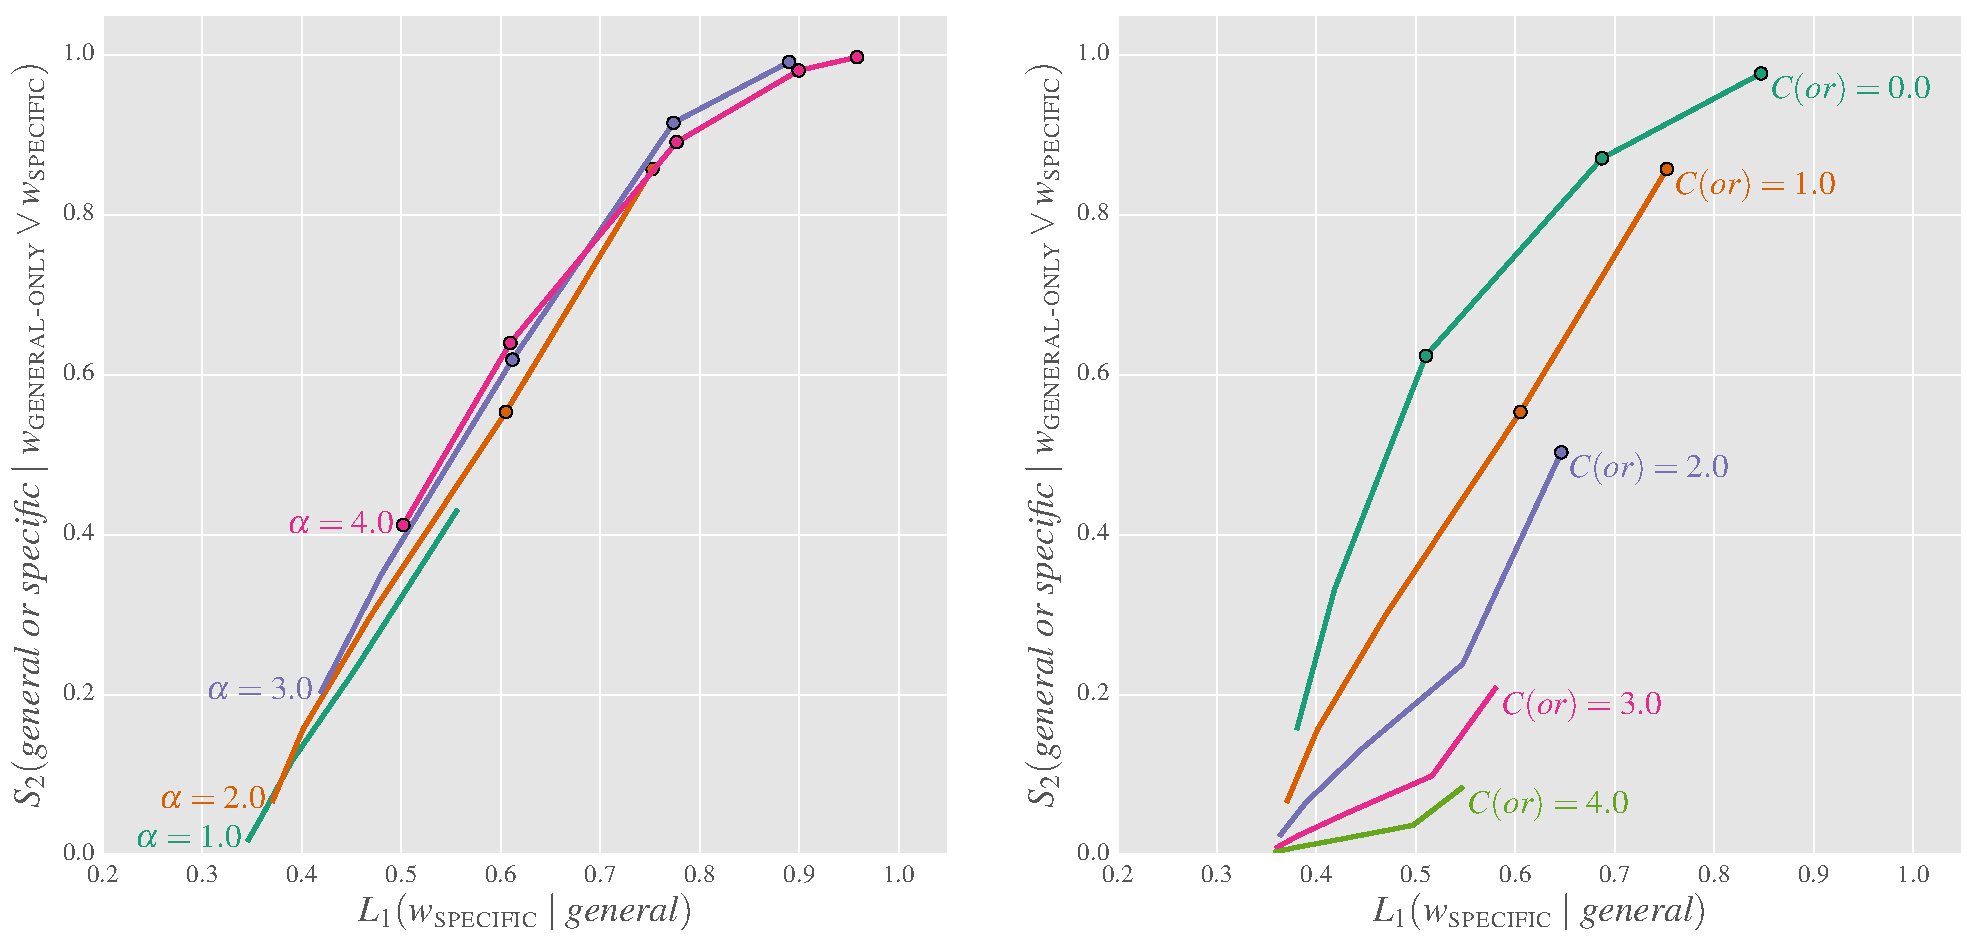
\includegraphics[width=1\textwidth]{fig/Q-implicature-simulation}  
  \caption{Simulations of Q-implicature blocking. The x-axis variation is created
    by varying $\Costs(\word{specific})$ from $1$ to $4$, with lower
    costs corresponding to higher values (more implicature inferences
    from \word{general} to \word{not-specific}).  On the left, we hold
    $\Costs(\word{or}) =1$ and trace four different values of
    $\alpha$. On the right, we hold $\alpha=2$ and trace four values
    of $\Costs(\word{or})$.}
  \label{fig:qsims}
\end{figure}

The key mechanism for the above example is variation in the cost of
the specific term. To simulate I-implicatures, we instead vary the
prior likelihood of the referents. \Figref{fig:isims} summarizes the
picture abstractly. Here, we have a general term like \word{boat} and
two specific terms like \word{motorboat} and \word{canoe}, referring
to objects $r_{\textsc{common}}$ and $r_{\textsc{uncommon}}$,
respectively. This would correspond to a situation where we work at a
marina that is largely devoted to motorboats, with canoes infrequent
and not especially salient. As in \figref{fig:qsims}, the x-axis
tracks the inferences of $\ListenerK[1]$. We are now interested in
this agent's inference from hearing the general term (\word{boat}) to
the more frequent subkind as the referent. We obtain this variation by
varying the prior over $r_{\textsc{common}}$ from $0.33$ to $0.99$.
The y-axis shows $\SpeakerK[2]$'s responses given the disjunctive
observation $r_{\textsc{common}} \vee r_{\textsc{uncommon}}$. Dots on
the lines again correspond to places where violating HG with the
disjunction \word{general or marked\_specific} (e.g., \word{boat or
  canoe}) is the preferred utterance. Here again, $\alpha$ and the
cost of disjunction influence these speaker choices greatly.  For
instance, $1.06$ is approximately the lowest $\alpha$ that generates
this behavior, whereas high values of $\alpha$ make it more
likely. Conversely, high disjunction costs again reduce the number of
HG-violations by making them worthwhile for the speaker only if the
listener's tendency to draw I-implicatures is very high.

\begin{figure}[tp]
  \centering
  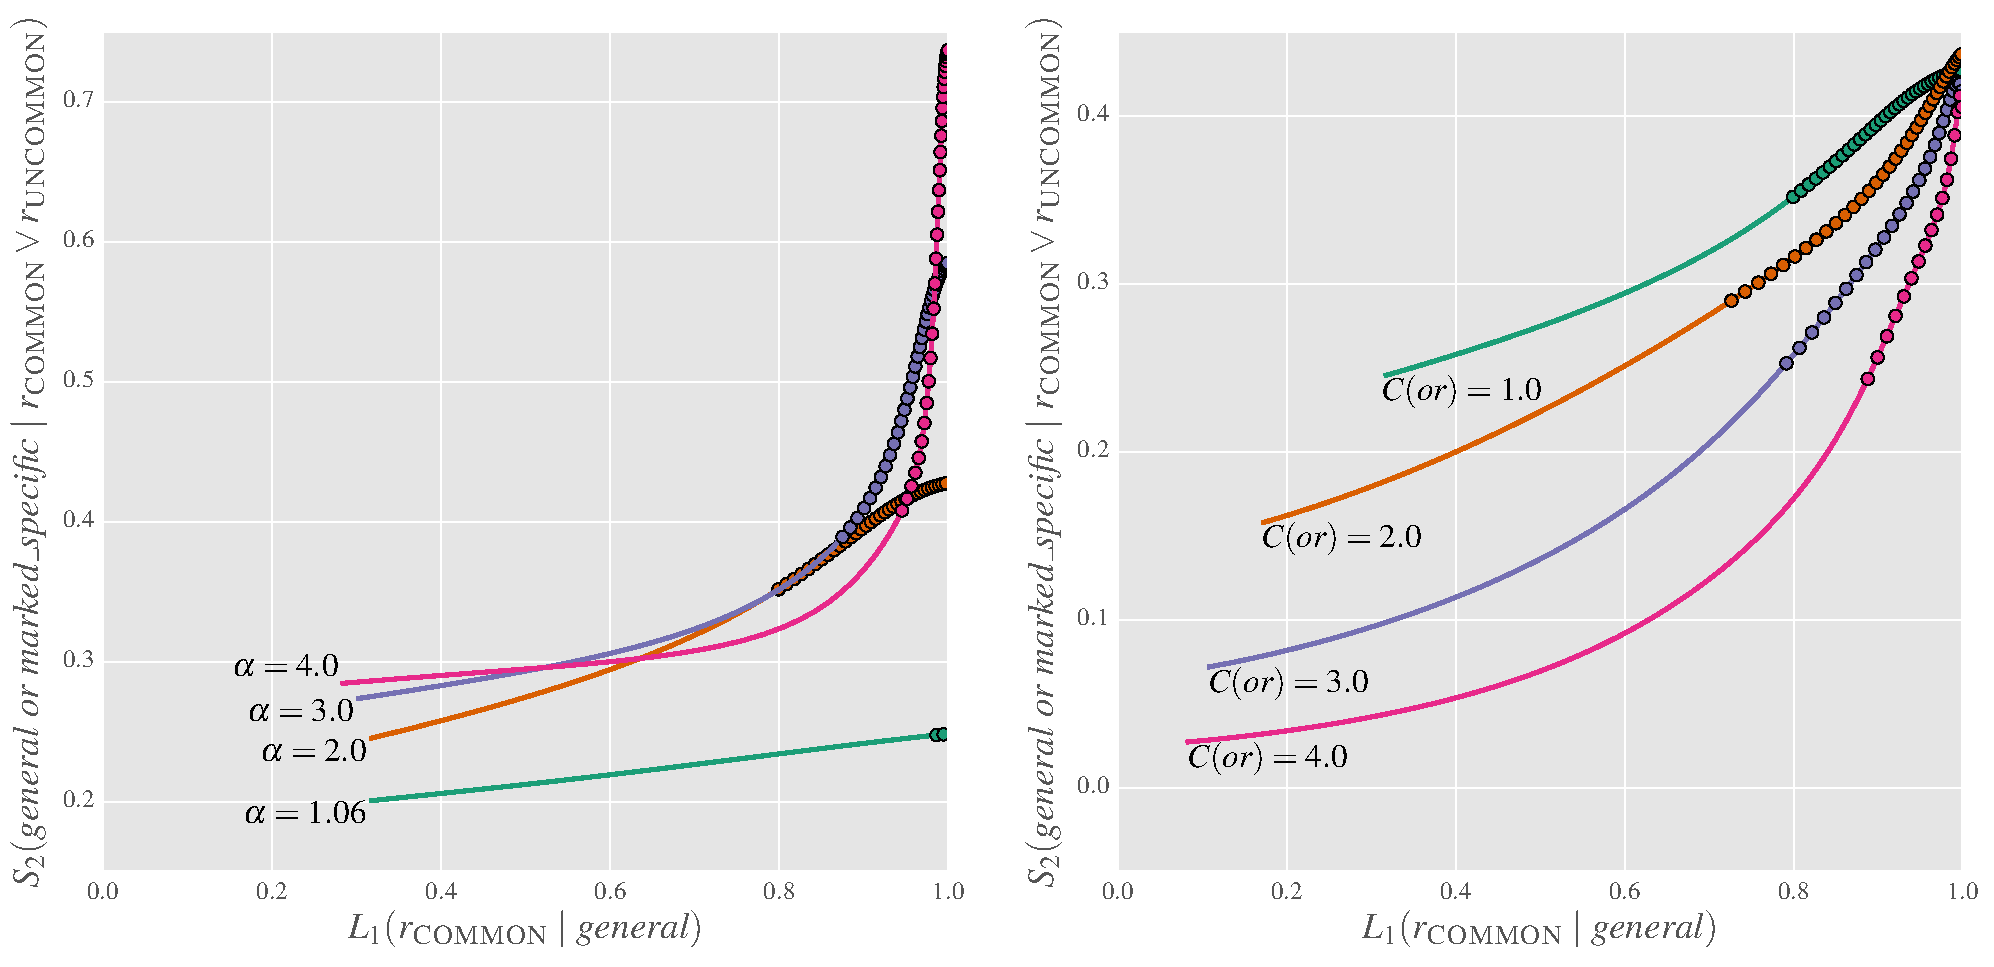
\includegraphics[width=1\textwidth]{fig/I-implicature-simulation}  
  \caption{Simulations of I-implicature blocking. The x-axis variation is created
    by varying $\Prior(r_{\word{common}}$ from $0.33$ to $0.99$, with
    higher values for this prior corresponding to higher listener
    inferences (more implicatures from \word{general} to
    \word{specific\_unmarked}).  On the left, we hold
    $\Costs(\word{or}) =1$ and trace four different values of
    $\alpha$. On the right, we hold $\alpha=2$ and trace four values
    of $\Costs(\word{or})$.}
  \label{fig:isims}
\end{figure}

The above simulations show that the model can simulate not only
implicature inferences but also the kind of behavior that would
normally be characterized as implicature blocking. This possibility
arises from the recursive nature of the model, in which pragmatic
speakers can anticipate the construals of pragmatic listeners and plan
their own utterances accordingly. We should emphasize also that
Q-implicature and I-implicature scenarios represented by
\figref{fig:qsims} and \figref{fig:isims} are just particular
examples. Since neither kind of implicature is a primitive of the
model, but rather just emerges from other interactions, we are not
limited to explanations that fall precisely into one of these two
categories, which aligns well with our intuitions about the complex
factors that guide HG violations in communication.

%=====================================================================

\subsection{Parameter space exploration}\label{sec:characterization}

The above illustrative examples provide initial clues as to how our
model characterizes Hurfordian and definitional uses from the speaker
and listener perspectives. The goal of this section is to more
thoroughly explore the space of options, with the goal of formulating
a meta-theory of these behaviors and their relationships to the facts.

As we discussed at the start of this section, both uses require the
speaker to be invested in some sense in communicating information
about the lexicon.  In a similar vein, the listener must have some
lexical uncertainty, or at least be willing to defer to the speaker's
preferences. Both of these forces are centered around the parameter
$\beta$, which controls both speaker and listener behavior because of
the recursive nature of the model. If $\beta$ is set to $0$, then the
lexica are not distinguished from one another, and we end up with a
system in which only information about the world is exchanged.

The above illustrative examples begin to show that $\beta$'s
relationship to the parameter $\alpha$ and the cost of disjunction are
what steer the discourse participants to exclusivization or
identification. \Figref{fig:char} gives a fuller picture of these
dynamics using our larger lexicon setting (five atomic messages, four
atomic states). The x-axis gives $\log(\beta/\alpha)$ for values of
$\alpha$ and $\beta$ between $0$ and $14$ inclusive, in increments of
$1$. The log-scale helps bring out the underlying relationships, and
it also means that values above $0$ are where $\beta$ is bigger than
$\alpha$. The y-axis gives the cost of disjunction, ranging from $0$
to $0.2$, in increments of $0.01$. The dots classify best inferences in
this space of parameters, with green marking strictly dominant Hurford
strategies, orange marking strictly dominant definitional strategies,
and purple marking cases where both strategies are strictly dominant
(which is possible because we've reduced $\alpha$ and $\beta$ to a
single measure in order to visualize the space in two dimensions).

\begin{figure}[tp]
  \centering
  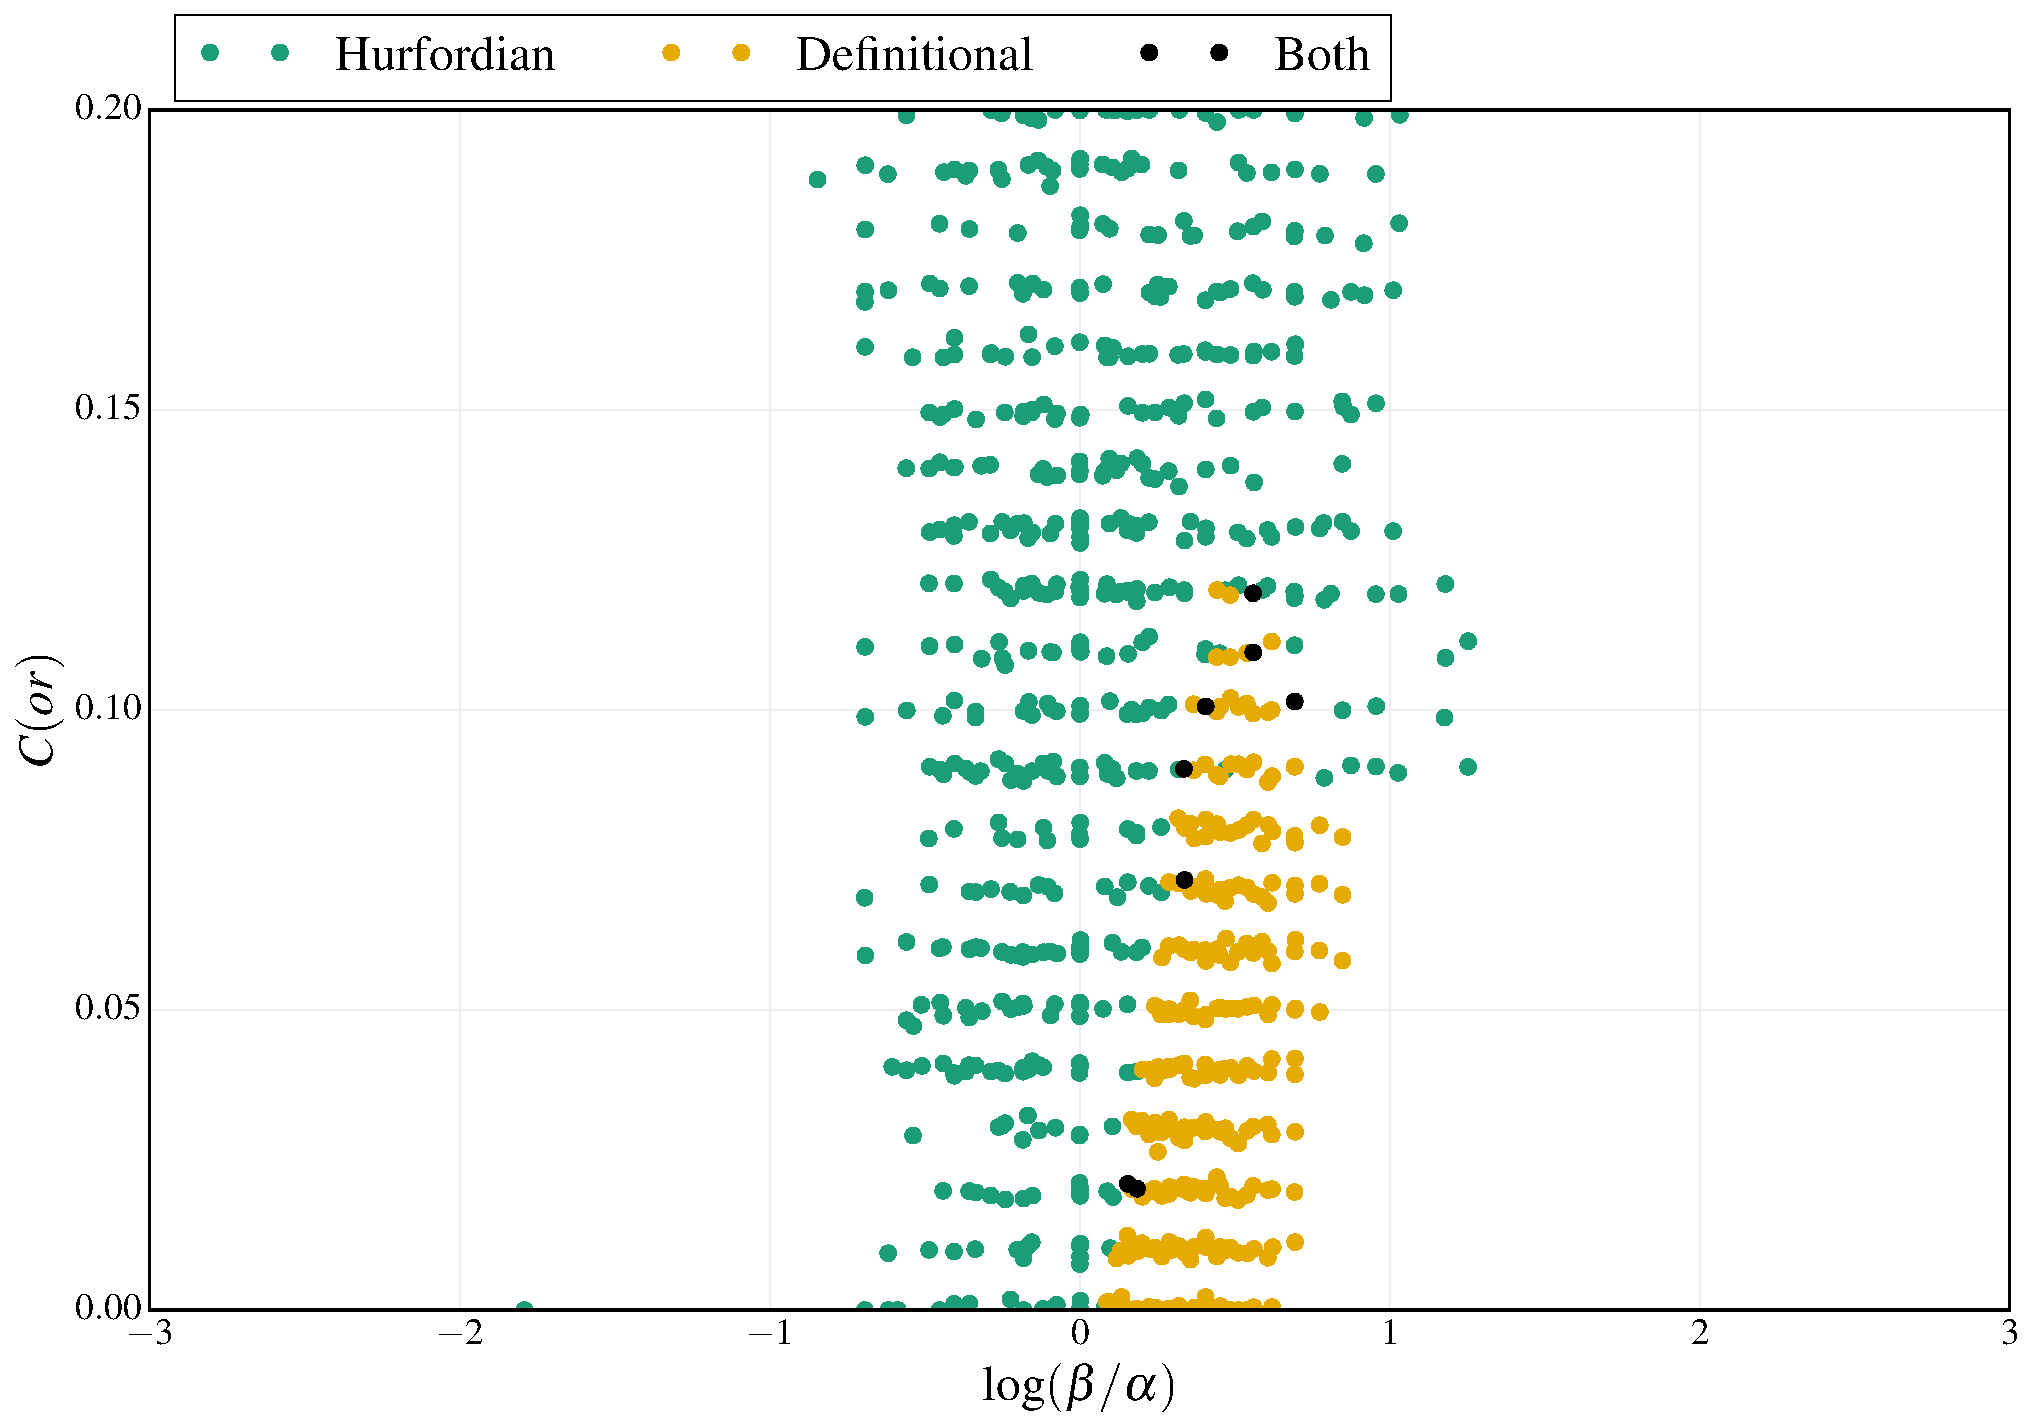
\includegraphics[width=0.8\textwidth]{fig/paramexplore-lex5}
  \caption{Hurfordian and definitional contexts with a large lexicon
    (five atomic lexical items, four atomic states).}
  \label{fig:char}
\end{figure}

\begin{figure}[tp]
  \centering
  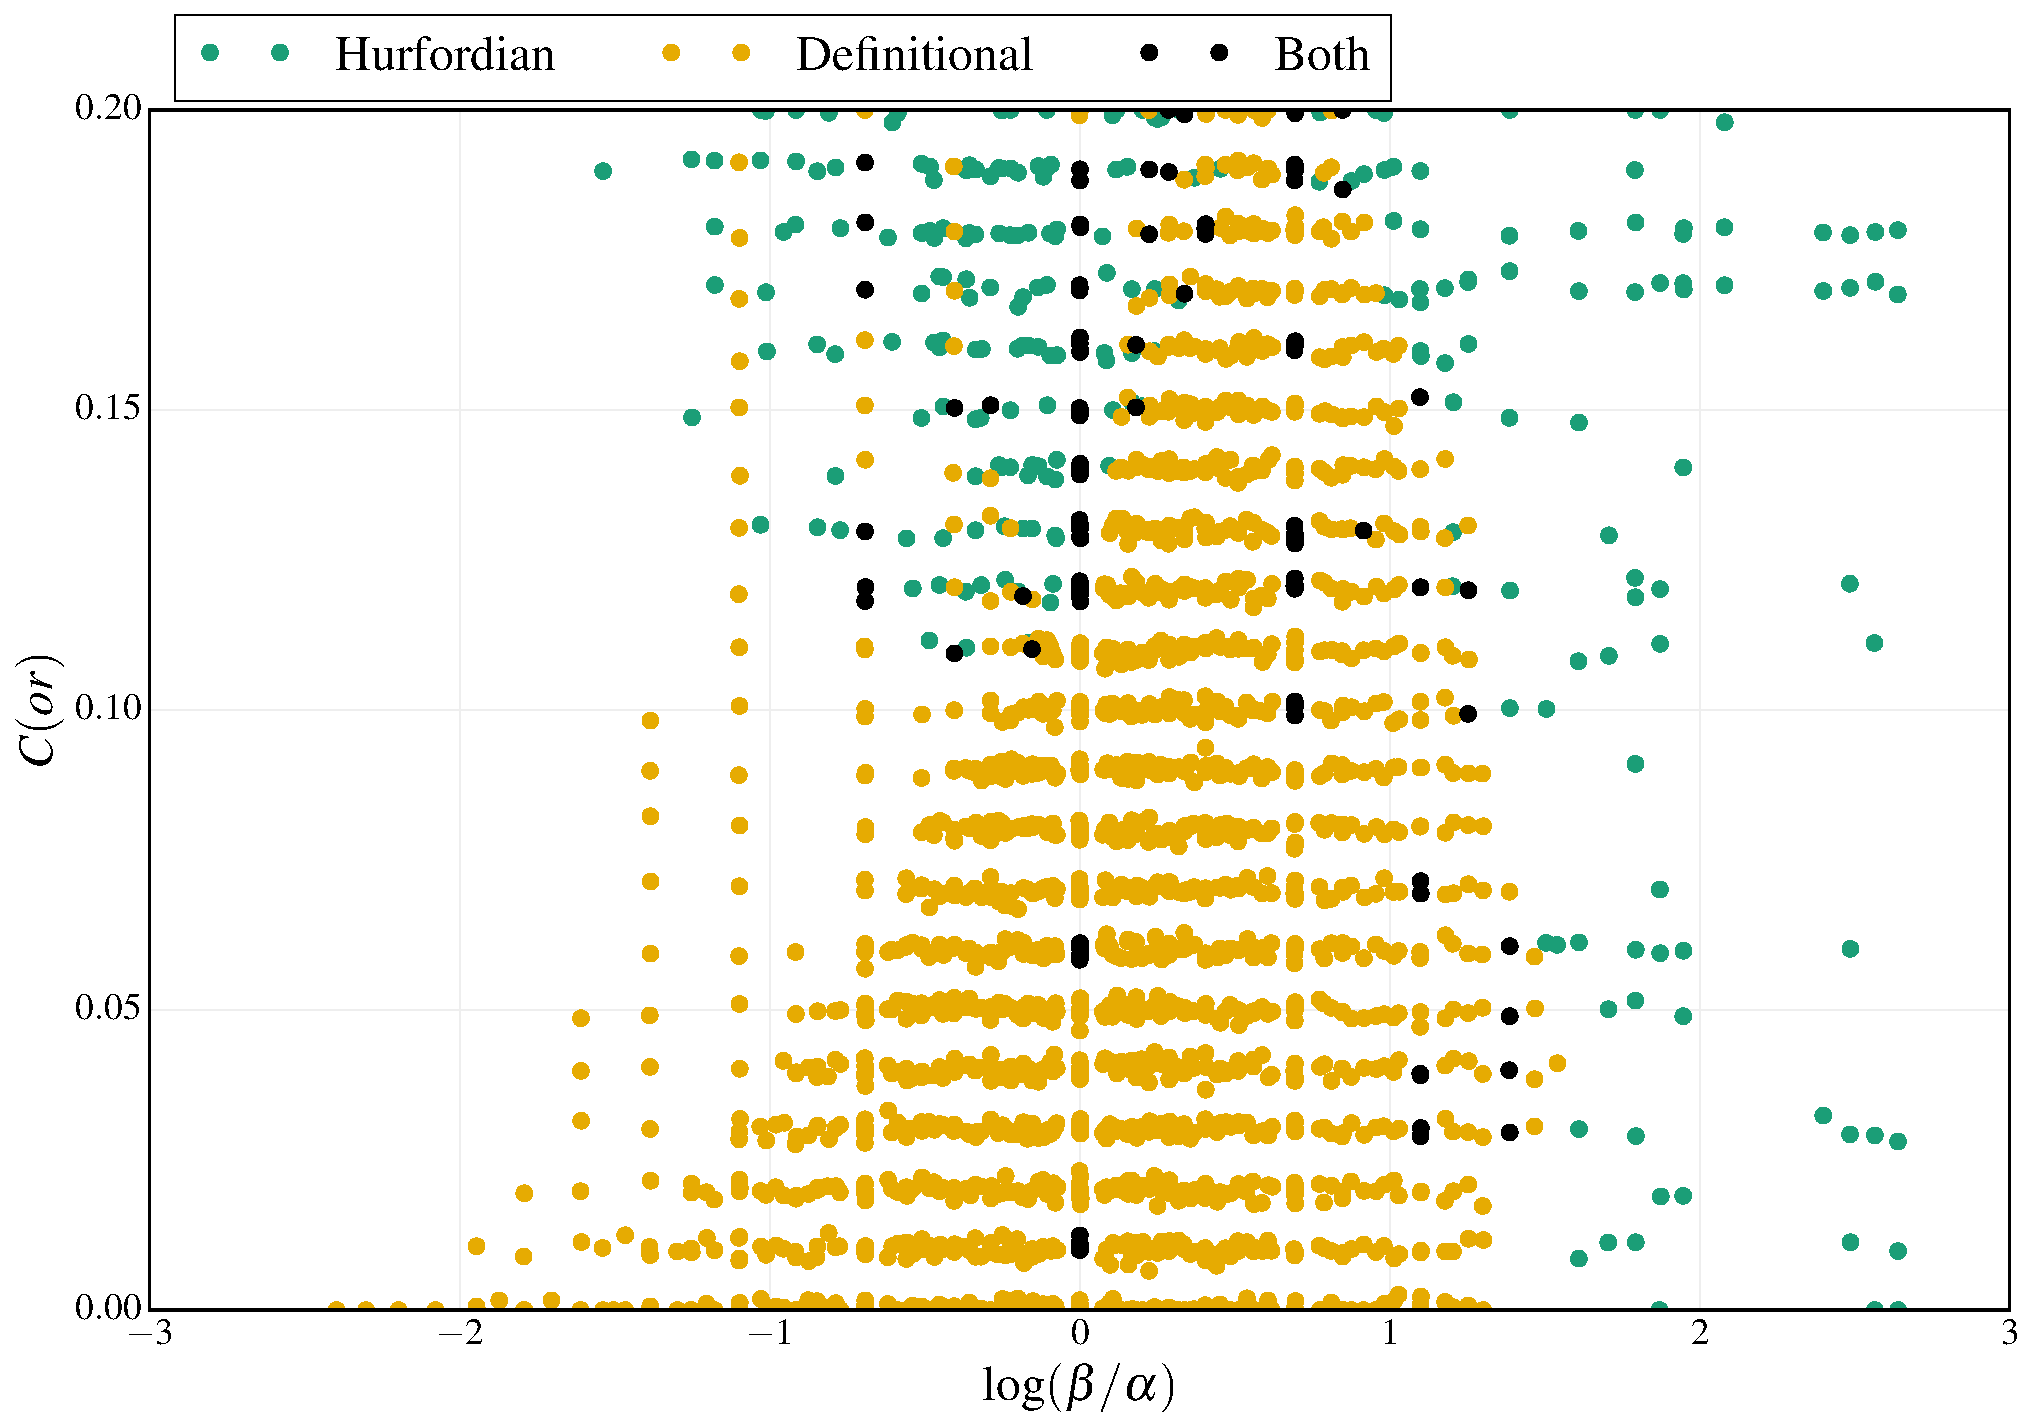
\includegraphics[width=0.8\textwidth]{fig/paramexplore-lex5-focal}
  \caption{A focal point unknown word. Hurfordian and definitional
    contexts with lexicon (five atomic lexical items, four atomic
    states).}
  \label{fig:char-focal}
\end{figure}

The picture that emerges from \figref{fig:char} is relatively clear:
definitional readings exist in a narrow space where $\beta > \alpha$
and disjunction costs are low. (Very small lexica and world spaces are
somewhat more lenient about this, but it seems to hold in systems of
sufficient complexity to allow meaningful adjustments to the
messages.) As we said above, this makes intuitive sense: where costs
are high, the disjunction has to be justified. Letting the two terms
overlap reduces the justification, whereas exclusivizing provides
justification with regard to $\alpha$. However, the pressures of
$\beta$ also intrude. If $\beta$ is high, then it might be worth
paying the disjunction costs for the sake of teaching the listener
about the lexicon, even if this reduces the amount of information
conveyed per word.

From this perspective, it is clear why Hurfordian uses are more
robust. They arise in a much wider range of contexts because they can
easily survive high disjunction costs --- exclusivization ensures
genuine communicative value. In contrast, definitional readings exist
mainly in the space of low disjunction and high $\beta$ because the
state information they convey is fully encoded in the first disjunct,
making the full disjunction an inefficient way of conveying world
information.

The quantitative picture also leads us to expect that there can be
uncertainty about whether the listener should regard the disjunction
as definitional or Hurfordian. The discourse participants might be in
a blurry area in which small changes to the parameter settings push
towards one inference or the other, with the difference between the
best and next-best inferences relatively small. This can persist even
when one of the words is unknown to the listener. (In such cases, the
disjunctive meaning is just extremely general and will not do justice
to the speaker's intentions.)

We saw in \secref{sec:analysis:definitional} that constraining the
unknown word to have an atomic meaning --- a meaning at the same level
of specificity as the other lexical items --- can greatly increase the
strength of the definitional inference.  \Figref{fig:char-focal} shows
that this is also reflected in the full parameter space. The figure is
based on the same data as \figref{fig:char} but with the focal point
assumption constraining the space of lexica. The result is that
definitional readings now exist in a much wider area of the parameter
space: disjunction costs can be higher and $\beta$ can be smaller than
$\alpha$. Thus, if a context supports this general constraint --- for
example, if the speaker is known to be trying to instruct the listener
about words and concepts --- then definitional readings should be more
salient.


%%%%%%%%%%%%%%%%%%%%%%%%%%%%%%%%%%%%%%%%%%%%%%%%%%%%%%%%%%%%%%%%%%%%%%

\section{Conclusion}\label{sec:conclusion}

This paper synthesized and extended ideas from recent models of
language production and construal, especially those of
\citet{Smith:Goodman:Frank:2013} and \citet{bergen-levy-goodman:2014},
in order to provide a unified account of two seemingly conflicting
inferences that disjunction supports --- a pressure to exclusivize the
disjuncts and a pressure to regard them as synonymous.  From a single
model of disjunctive semantics coupled with general principles of
pragmatic inference, a rich variety of uses of disjunction emerge:
definitional interpretations
(Section~\ref{sec:analysis:definitional}), Hurfordian exclusivization
interpretations (Section~\ref{sec:analysis:subsumptive}), and
defensive, implicature-blocking speaker behavior
(Section~\ref{sec:defensive-speakers}).  Each use within this rich
variety traces to a specific set of relative priorities of the
discourse participants with regard to communicating about the language
itself, communicating about the world, and avoiding or tolerating
undue message costs.

Our most fundamental contributions lie in the structure of the
pragmatic model. We allow the speaker's communicative intentions to
include linguistic preferences, and we allow listeners to make
inferences about those preferences during the regular course of
linguistic interactions. This structure is particularly important for
exclusivization inferences, which do not affect truth conditions and
so do not even emerge in most models.  We hope this approach suggests
new ways of detecting and understanding the secondary messages encoded
in speakers' utterances, and that it can shed new light on the
importance of communicating in language about language, and on related
issues involving meta-linguistic negotiations and variable levels of
perceived expertise about the language. More broadly, it could also
serve as a way to connect pragmatic inference with phenomena relating
to linguistic change and pedagogy, social identity, social
hierarchies, and linguistic style.

%%%%%%%%%%%%%%%%%%%%%%%%%%%%%%%%%%%%%%%%%%%%%%%%%%%%%%%%%%%%%%%%%%%%%%

\bibliographystyle{language}
\bibliography{PottsLevy_BLS41-bib.bib}

\end{document}

